%!TEX root = ../main.tex
\chapter{Improving the Robustness of Cyber-Physical System Models}
\label{ch:CPSRobustness}
\begin{quote}
    "Attacks are random faults that are not really random." -- Carlos Murguia.  
\end{quote}
\todo[inline]{Here comes the paper we are going to send to TOPS. I am not going to put it here to prevent duplication and inconsistencies.}

\section{Introduction}
\todo[inline]{@John: you can probably provide a more exciting introduction to CPSs and why attacks on CPS are very problematic. We are trying to answer the question: why did you choose CPSs for this analysis?}
\todo[inline]{@John: I guess we should make some specific emphasis on why physical components are critical}
{\color{red}
A \emph{cyber-physical system} (CPS) is a system that intertwines components from the physical and digital worlds. Some examples of CPSs include: cars, aircrafts, water treatment plants, industrial control systems, and critical infrastructures. Security violations in a safety-critical CPS has notable effects in the physical world, \emph{e.g.,} in late 2007 or early 2008, the Stuxnet attack against an Iranian control system allegedly sabotaged centrifuges in uranium enrichment plants, causing them to rapidly deteriorate \cite{StuxnetWeb,Stuxnet}, and in 2014, hackers struck a steel mill in Germany and disrupted the control system, which prevented a blast furnace from properly shutting down, causing massive damage to the facility \cite{WiredArticle,Lagebericht2014}.
}
\todo[inline]{@John: we want to motivate studying integrity for CPS. Actually, we would be more interested in robustness. Do you have good definitions of what robustness is that we can cite? Robustness, as I understand it, quantifies some aspects of integrity, and resilience quantifies other aspects.}
{\color{red}
Although in the scientific literature on information security \emph{confidentiality} has traditionally enjoyed more attention than \emph{integrity}, as observed for instance by Clark and Wilson \cite{ClarkWilson87}: ``in the commercial environment, preventing disclosure is often important, but preventing unauthorized data modification is usually paramount.''
This holds particularly true for many Industrial Control Systems (ICSs) at yet another level: their security priority is not the protection of confidential data, but the protection of their physical assets.  Gollmann and Krotofil reinforce this paradigm in \cite{CPSSec}, stating that the traditional CIA (Confidentiality-Integrity-Availability) triad should be reversed when studying the security of CPSs. They argue that the enforcement of integrity in CPSs should not only consider the ``traditional approach for IT systems'', \emph{i.e.}, protecting \emph{component logic} and \emph{communication}, but that we must also protect the integrity of {observations}; more precisely, we have to protect the \emph{veracity} of sensor data and check its \emph{plausibility}.}

{Traditionally, the enforcement of CPS integrity has focused on guaranteeing that systems perform as their designers intended. This is usually evaluated using {control-theoretic methodologies}, specifically {fault-detection techniques}. Control theory researchers model attacks to CPSs as time-series with specific structures affecting sensor measurements and/or control signals. Depending on their capabilities, attackers have the power to control when, where, and how attacks are induced to the system. Research on attack detection and mitigation has mainly focused on the so-called \emph{integrity attacks}, i.e., attacks that put at risk the proper operation and physical integrity of CPSs. Integrity attacks include stealthy attacks \cite{CPSStealthAttacks}, message replay \cite{CPSReplayAttacks}, covert attacks \cite{CPSCovertAttacks}, and false-data injection \cite{CPSDataInjectionAttacks}, among others. Due to their focus on fault-detection techniques, many results based on control theory aim to protect CPSs from integrity attacks in two ways: one, by first verifying that their system satisfies a series of security guarantees during normal operation, and second, by relying on {monitoring} the physics of the system to detect anomalies (see, e.g., \cite{CPSInvariantsForDetection,LimitingImpactStealthyAttacks,CPSAttackDetection,CPSAttacksAgainstPCS,CPSIntegrityAttacks,CPSDetectingIntegrityAttacksScada}).
}

{%\color{red}
In sum, most control-theoretical approaches to CPS security assume the existence of a probabilistic behavioural model that is used as a reference of normal (attack-free) behaviour, and their goal is to monitor and protect the system with respect to this ideal model at runtime, when attacks might arise. There are some limitations with this approach. On the one hand, this approach is mainly reactive, and as such it does not shed light on how to improve a given CPSs design in order to make it more robust (although there are some recent results on {redesigning controllers and models} to improve robustness of CPSs against attacks, e.g., \cite{Carlos_Justin3,Weerakkody}). On the other hand, an inherent limitation of many behavioural models for CPS is that they usually are approximate due to linearisation, and might produce a high false-positive rate when used in practice; moreover, some works (e.g., \cite{LimitingImpactStealthyAttacks,CPSDetectingIntegrityAttacksScada,IFCPSSec}) rely on the assumption that it is possible to determine whether the system is operating normally or under attack, but there could be non-malicious deviations of a given behavioural model due to routine maintenance operations or other random benign factors. Finally, only few approaches (such as \cite{IFCPSSec,Gupta2,Carlos_Justin3}) quantify the severity and consequences of attacks on the system.%,
}
%\todo[inline]{@ALL: let me try to sell the latent behaviour analysis method to you. If you think this following argument is weak, please let me know. }

\todo[inline]{Describe that fault injection is naturally used to find robustness problems.}

In this work, we suggest using the same techniques we have for fault injection, but reversing the roles: we apply fault injection on vulnerable systems to try to compensate for the actions of attackers, and to give designers of CPSs an intuition of how to make their systems more robust.

Abstractly, an attack $m$ is a fault purposely injected by an attacker. The attack $m$, in a way, transform the system, and causes it to behave differently. 
\todo[inline]{Complete}

\emph{Latent behaviour analysis} is the study systems with respect to a behavioural variable $m$ which transforms the normal behaviour of the system. As we vary $m$, we characterise different behaviours realisable by the system. In the context of fault injection, every fault $m$ acts as a system transformation whose objective is destructive; i.e., $m$ stresses the system so it fails its security requirements. However, we can turn the roles around, and try to find a set of ``counter-faults'' which invalidate $m$. We can then give the set of counter faults to the designer so that they can use them as a starting point for redesigning reaction mechanisms for when an attack is detected. 

If we model the behaviour of a CPS as a function $\TheSystem\colon\Pi\rightarrow\Pi$, where $\Pi$ is the set of states, which evolves the state of the system over time, we can compose $\TheSystem$ with a state transformation $m\colon \Pi\rightarrow\Pi$ and reveal a behaviour $\TheSystem\circ m\colon\Pi\rightarrow\Pi$. We call $\TheSystem\circ m$ the \emph{latent behaviour revealed by $m$}, because it depends on the behavioural variable $m$. The normal behaviour of the system corresponds to the latent behaviour revealed by the identity transformation, since $\TheSystem\circ \id=\TheSystem$. If $m$ models an attack, then we can introduce an additional behavioural variable $w$ to reveal an additional latent behaviour $\TheSystem\circ w\circ m$, and if $w$ counters the actions of $m$, then we could use $w$ constructively instead of destructively to implement contingency methods for when the attack $m$ is detected via runtime monitors.

Theoretically, if the set of states $\Pi$ is finite, there are $|\Pi|^{|\Pi|}$ possible values for the latent variables $m$ and $w$.  However, in the case of $m$, this set of transformations models an attacker that is capable of arbitrarily morphing the state of the CPS, including both cyber and physical aspects, in any form and at any time. This attacker is trivially too powerful to defend against, not to mention impractical, since it can in theory bypass physical invariants (e.g. Boyle's law). In this work, we show how to systematically generate a set of transformations $m$ which represent realistic and practical attacks. We use the revealed latent behaviours $\TheSystem\circ m$ to quantify the robustness of the system in the same spirit as fault injection. Then, because attacks and counter-attacks are duals of the same type, we use a similarly-generated of transformations to try to find, for each attack $m\colon\Pi\rightarrow\Pi$, a counter-attack $w\colon\Pi\rightarrow\Pi$. Each attack+counter-attack pair can give the designer of the CPS useful insights on how to make the control strategy more robust and how to implement mitigation mechanisms that are more effective.

% Formally, any transformation $m\colon\Pi\rightarrow\Pi$ can be used to reveal a latent behaviour. 
% However, we are interested in those $m$ that model realistic attacks. 
% In this work, we provide a framework to define attacks and attackers, and a method to systematically generate them, yielding a universe $\mathcal{A}$ of attackers and a universe $\mathcal{M}$ of attacks.
% , and two mappings between them: 
% the mapping $\texttt{has}\colon\mathcal{A}\rightarrow\mathscr{P}(\mathcal{M})$ which maps each attacker to the set of attacks they can perform, and a mapping $\texttt{minimal}\colon\mathcal{M}\rightarrow \mathcal{A}$, which maps each attack to the attacker with minimal capabilities that can perform it.
To estimate the robustness of a system, we need a notion of success for attacks and attackers. For such purpose, assume the existence of a set of security requirements $\TheSetOfRequirements$. 
We consider a system to be robust with respect to a universe of attacks $\mathcal{M}$ if no attack in $\mathcal{M}$ can break any security requirement in $\TheSetOfRequirements$. 
However, while it is expected that the system under normal circumstances satisfies all security requirements in $\TheSetOfRequirements$, it is not unexpected that the system fails to satisfy some security requirement while it is under attack. 
\todo[inline]{@Martin: because we expect the latent behaviours to fail at least one requirement, it is more efficient to test them than it is to verify them. The tools you provided are excellent for verification, but we are much better with runtime monitors and simulations. }
\todo[inline]{@All: at the end of the motivational example I put a list that summarises what this paper is and what this paper isn't. I hope that helps define the focus of this paper. If you agree with that list, then it is easier to write the contributions and disclaimers.}
% \todo[inline]{@Eric: explain what it means for a system to be robust and how to quantify its robustness.}
% \todo[inline]{Here is where i'm a bit stuck and why it is important to do some experiments. I'm working together with John and Sudipta to define interesting use cases for our Latent behaviour analysis (LBA)}
%Instead of determining whether a system is secure or not, we are interested in the following decision problem: given two candidate designs of system, decide which one is more secure.% and determining what aspects of the system require more urgent redesign. 
%  the set $\texttt{Vulnerabilities}\subseteq $, of attacks that can break a security requirement, and a metric for attackers, named $\texttt{flexibility}\colon \mathcal{A}\rightarrow \mathscr{P}(\mathcal{M})$ which maps each attacker to the set of their successful attacks (i.e. attacks that can break at least one security requirement). 

% In this work, we measure the security of the system by counting the number of attacks that are successful.

%%%%%%%%%%%%%%%%%%%%%%%%%%%%%%%%%%%%%%%%%%
%          Chemical toy example
%\input{old_sections/old_Introduction} 
%%%%%%%%%%%%%%%%%%%%%%%%%%%%%%%%%%%%%%%%%%
{\color{red}
\todo[inline]{@Eric: Update this discussion. The problem statement is similar, but the approach is quite different.}
\textbf{Problem statement:} To summarize, in this work we address the following
questions: \emph{Can we identify at design time which inputs to a CPS are most
harmful if controlled by an attacker? Can we improve the design of the CPS
at design time and justify our models formally with respect to a precise
integrity notion?}

\textbf{Approach:} We propose to model a CPS as a composition of the control
logic and the expected systems behaviour in terms of a finite and deterministic
state machine. We then formally quantify the impact of various attackers
(controlling physical or logical aspects of the system) to the integrity
of critical physical states by means of information flow analysis.

\textbf{Contributions:} We make the following contributions \textbf{a)} We present a logical framework to formally reason about integrity in CPS models,
reconciling information flow analysis and control theoretical aspects. \textbf{b)} We discuss how our approach can be used to spot and quantify harmful information flows in CPS. \textbf{c)} We illustrate the usefulness of
our approach by means of simple but realistic models concerning a water
distribution CPS and show that we can identify non-trivial integrity-harming flows
in a CPS.
}
{
\section{Control Theory Preliminaries}
% \todo[inline]{Do we really need to present control theory preliminaries? Or is there an IT approach to CPS attacks?}
Gollmann and Krotofil highlight, ``to work on cyber-physical systems, one has to combine the devious mind of the security expert with the technical expertise of the control engineer''~\cite{CPSSec}. 
Unfortunately, this expertise is ``not commonly found in the IT security community''~\cite{CPSSecVinyl}. 
% according to the authors of  
Moreover, the language barrier between control theory and IT security disciplines worsens this lack of expertise.
Thus, in this section, we present the model-based techniques for CPSs security broadly used by the systems and control community.
\subsection{Linear Time-Invariant Models.}
During the last decade, there has been an increasing tendency to use physics-based models of CPSs to detect and quantify the effect of attacks on the system performance \cite{CPSAttacksAgainstPCS,LimitingImpactStealthyAttacks,CPSDetectingIntegrityAttacksScada,CPSIntegrityAttacks,Carlos_Justin1,Carlos_Justin2,Carlos_Justin3}. These physics-based models focus on the normal operation of the CPS and work as prediction models that are used to confirm that control commands and measurements are valid and plausible. Often, dynamical models of physical systems are approximated around their operation points or approximated using input-output data. These lead to approximated models which are often linear and time-invariant.

Following the work in \cite{CPSAttacksAgainstPCS,LimitingImpactStealthyAttacks,CPSDetectingIntegrityAttacksScada,CPSIntegrityAttacks,Carlos_Justin1,Carlos_Justin2,Carlos_Justin3}, here, we only consider Linear-Time Invariant (LTI) models, although the same ideas are employed when considering more complicated dynamics. In particular, a model of a CPS that uses LTI stochastic difference equations is of the form
\begin{equation}
\left\{
\begin{array}{ll}
{x}({k+1}) = Ax(k) + B u(k) + \vartheta(k),  \label{1} \\[1mm]
\hspace{3.8mm} y(k) = Cx(k) + \eta(k),
\end{array}
\right.
\end{equation}
with $k\in \Nat$, physical state of the system $x \in \Real^n$ (i.e., an $n$-dimensional vector of physical variables associated with the dynamics of the CPS), sensor measurements $y := (y_1,\ldots,y_m)^T \in \Real^m$ , control signals $u := (u_1,\ldots,u_m)^T \in \Real^l$, real-valued matrices $A$, $B$, and $C$ of appropriate dimensions, and i.i.d. multivariate zero-mean Gaussian noises $\vartheta \in \Real^n$ and $\eta \in \Real^m$ with covariance matrices $R_{1} \in \Real^{n \times n}$ and $R_2 \in \Real^{m \times m}$, respectively. The matrix $A$ describes the \emph{dynamic evolution of the physical process}, $B$ is used to model the effect of \emph{actuators} on the system dynamics, and the matrix $C$ models the part of the state $x_k$ available from \emph{sensor measurements}.

\subsection{Attacks on Models of CPSs}
\label{sec:AttacksOnModels} 
At the time-instants $k \in \Nat$, the output of the process $y(k)$ is sampled and transmitted over a communication network. The received output is used to compute control actions $u(k)$ which are sent back to the physical process. The complete control-loop is assumed to be performed instantaneously, i.e., the sampling, transmission, and arrival time-instants are supposed to be equal.
In between transmission and reception of sensor data and control commands, an attacker may replace the signals coming from the sensors to the controller and from the controller to the actuators, acting as a \emph{Man-in-the-Middle}. Thus, after each transmission and reception, the attacked output $\bar{y}$ and attacked input $\bar{u}$ take the form
\begin{equation}
\left\{
\begin{array}{ll}
\bar{y}(k) := y(k) + \delta^y(k) 
, \label{3}\\[1mm]
\bar{u}(k) := u(k) + \delta^u(k),
\end{array}\right.
\end{equation}
where $\delta^y(k) \in \Real^m$ and $\delta^u(k) \in \Real^l$ denote \emph{additive sensor and actuator attacks}, respectively.

%Henceforth, we denote $x(k)$ by $x_k$, $ \bar{u}(k)$ by $\bar{u}_k$, $\vartheta(k)$ by $\vartheta_k$, $\bar{y}(k)$ by $\bar{y}_k$, $\eta(k)$ by $\eta_k$, $\delta^y(k)$ by $\delta_k^y$, and $\delta^u(k)$ by $\delta^u_k$. Then, a
A system under attack is modelled by
\begin{equation}
% \left\{
% \begin{array}{ll}
% {x}_{k+1} = A x_k + B (u_k + \delta^u_k) + \vartheta_k,\label{17} \\
% \text{ \ \ }\hspace{.35mm}\bar{y}_k = C x_k + \eta_k + \delta^y_k.
% \end{array}
% \right.
\left\{
\begin{array}{ll}
{x}({k+1}) = A x(k) + B (u(k) + \delta^u(k)) + \vartheta(k),\label{17} \\
\text{ \ \ }\hspace{.35mm}{y}(k) = C x(k) + \eta(k) + \delta^y(k).
\end{array}
\right.
\end{equation}
For the interested reader, we include some extra material about these techniques in the appendix.
}
\section{Motivational Example}
\label{sec:example}
In this section, we provide a simple example to motivate the problem of quantifying robustness via testing in CPS models. We also illustrate the concepts behind the modelling formalisms presented in the following sections.

\todo[inline]{@John: Please add a super short description of what Stage 3 is about. JH: I suggest to explain the motivational example by itself, without mentioning it is part of SWaT, then we can keep it simple for the reader. Later when we introduce SWaT, we can say Stage3 is similar to the motivational example.}
%==================BEGIN JOHN WORKSPACE====================

%==================END JOHN WORKSPACE====================
In this section, we model SWaT's Stage 3 process as a LTI system, and we describe attackers for it in the traditional sense (i.e. attackers on its sensors and actuators)...
\todo[inline]{@Eric: Complete when this section is finished.}
\subsection*{A LTI Model of Stage 3}
To quantify the robustness of a CPS, we first need to define its model. Let $\vec{x}$ be the physical state vector, whose coordinates are $MV$, $L$ and $P$, such that $\vec{x}[MV]$ corresponds to the physical state of the motor valve, $\vec{x}[P]$ corresponds to the physical state of the pump, and $\vec{x}[L]$  corresponds to the physical state of the water level of the tank. The variable $\vec{x}[MV]$ can take four values: $\texttt{closed}, \texttt{opening},\texttt{open},$ or $\texttt{closing}$; the variable $\vec{x}[P]$ can take two values: $\texttt{on}$ and $\texttt{off}$; and the variable $\vec{x}[L]$ can take any value between $0 ~\mathrm{L}$ and $1200 ~\mathrm{L}$ (the maximum capacity of the tank). 
 
%\begin{figure}[t]
%\begin{wrapfigure}[lineheight]{position}{width}
\begin{wrapfigure}{r}{0.5\textwidth}
  \centering
  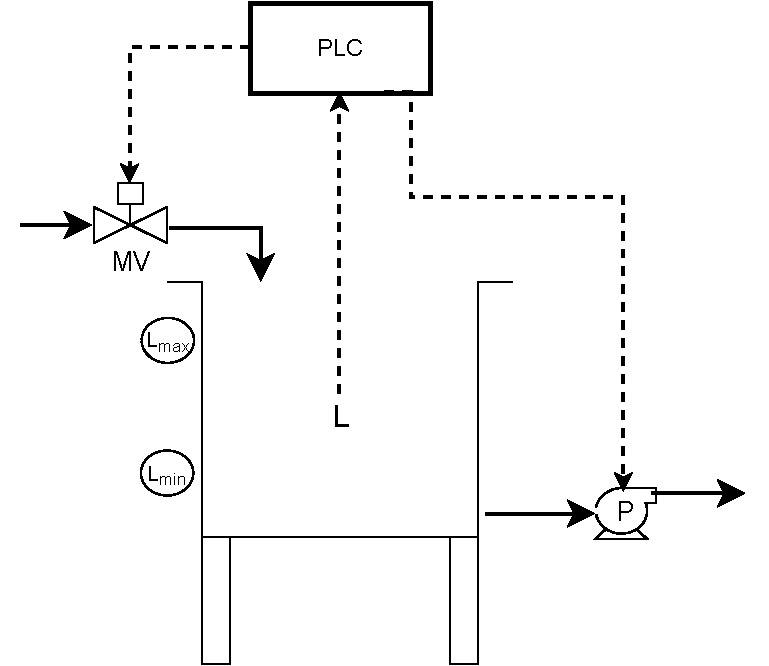
\includegraphics[width=0.36\textwidth]{Figures/FillingTank.pdf}
  \caption{Motivational example}
  \label{fig:Motivational}
\end{wrapfigure}
%\end{figure}

Depending on the state of $\vec{x}[MV]$, different amounts of water flow into the tank, so $\vec{x}[L]$ depends on $\vec{x}[MV]$. The state of the valve $\vec{x}[MV]$ changes when it receives a control input $\vec{u}[MV]$. The control input $\vec{u}[MV]$ can take the values $\texttt{closed}, \texttt{opening},\texttt{open},$ or $\texttt{closing}$. Finally, the state of the sensor $\vec{y}[L]$ is a measure of $\vec{x}[L]$; $\vec{y}[L]$ can take any positive value (even above 1200), although in normal circumstances it remains in the range $[0..1200]$. 

The behaviour of this process is captured by the following linear time invariant system.
\begin{align}
  \vec{x}[L](k+1)&= \vec{x}[L](k)+Inflow(k)-Outflow(k),\quad \text{where}\\
  Inflow(k)&=\begin{cases}
    0.31,&\quad \text{if $\vec{x}[MV](k)=\texttt{open}$}\\
    0,&\quad \text{if $\vec{x}[MV](k)=\texttt{closed}$}\\
    0.26,&\quad \text{otherwise}\\
  \end{cases}\\
  Outflow(k)&=\begin{cases}
    0.15,&\quad \text{if $\vec{x}[P](k)=\texttt{on}$}\\
    0,&\quad \text{otherwise}\\
  \end{cases}\\
    % \begin{cases}
    %   \vec{x}[L](k)+0.16,&\quad \text{if $(\vec{x}[MV](k),\vec{x}[P](k))=(\texttt{open}$,\texttt{on})}\\
    %   \vec{x}[L](k)-0.15,&\quad \text{if $\vec{x}[MV](k)=\texttt{closed}$,}\\
    %   \vec{x}[L](k)+0.11,&\quad \text{otherwise;}\\
    % \end{cases}\\
  \vec{x}[MV](k+1)&=\vec{u}[MV](k)\\
  \vec{x}[P](k+1)&=\vec{u}[P](k)\\
  \vec{y}[L](k)&=\vec{x}[L](k)
\end{align}
We leave the initial conditions of the process abstract for now.

The values of $\vec{u}[MV](k+1)$ are defined by a control strategy, which uses $\vec{y}[L](k)$ to make decisions. The control strategy is implemented by a controller whose state is $\vec{q}$, and $\vec{q}$ has four coordinates: the last known state of the valve $MV$, denoted by $\vec{q}[MV]$, the last known state of the pump $P$, denoted by $\vec{q}[P]$, the last known water level of the tank $L$, denoted by $\vec{q}[L]$,  and a timer $\tau$ which the controller uses to approximate the time it takes for the motor valve $MV$ to open or close, denoted $\vec{q}[\tau]$. 
The controller updates its state using $\vec{y}[L](k)$, and produces the next control values $\vec{u}[MV](k+1)$ and $\vec{u}[P](k+1)$ using $\vec{q}(k)$, with 
\begin{align}
  \label{eq:ControllerStager3}
  \vec{q}[MV](k+1)&=
  \begin{cases}
    \texttt{opening},&\quad \text{if $\vec{q}[MV](k)=\texttt{closed}$ and $\vec{y}[L](k)\leq Lmin$,}\\
    \texttt{open},&\quad \text{if $\vec{q}[MV](k)=\texttt{opening}$ and $\vec{q}[\tau](k)>T$,}\\
    \texttt{closing},&\quad \text{if $\vec{q}[MV](k)=\texttt{open}$ and $\vec{y}[L](k)\geq Lmax$,}\\
    \texttt{closed},&\quad \text{if $\vec{q}[MV](k)=\texttt{closing}$ and $\vec{q}[\tau_3](k) >T_3$,}\\
    MV&\quad \text{otherwise;}    
  \end{cases}\\
  \vec{q}[\tau](k+1)&=
\begin{cases}
  1+\vec{q}[\tau](k), &\quad \text{if $\vec{q}[MV](k)=\texttt{opening}$ or $\vec{q}[MV](k)=\texttt{closing}$}\\
  0,&\quad \text{otherwise;}    
\end{cases}\\
\vec{q}[L](k+1)&=\vec{y}[L](k)\\
\vec{q}[P](k+1)&=\texttt{on}\\
\vec{u}[MV](k+1)&=\vec{q}[MV](k+1)\\
\vec{u}[P](k+1)&=\vec{q}[P](k+1)
\end{align}
where $Lmin=800$, $Lmax=1000$ and $T=7$. We leave the initial conditions of $\vec{q}$ and $\vec{u}$ abstract for now.

Now that we have a description of the model of the CPS, we define a set of security requirements that determine whether the behaviour of the system is safe or not.

%\subsection{Security Requirements and Additive Attacks}
\subsection*{Security Requirements}
\begin{wrapfigure}{r}{0.4\textwidth} 
  \vspace{-1cm}
  \centering
  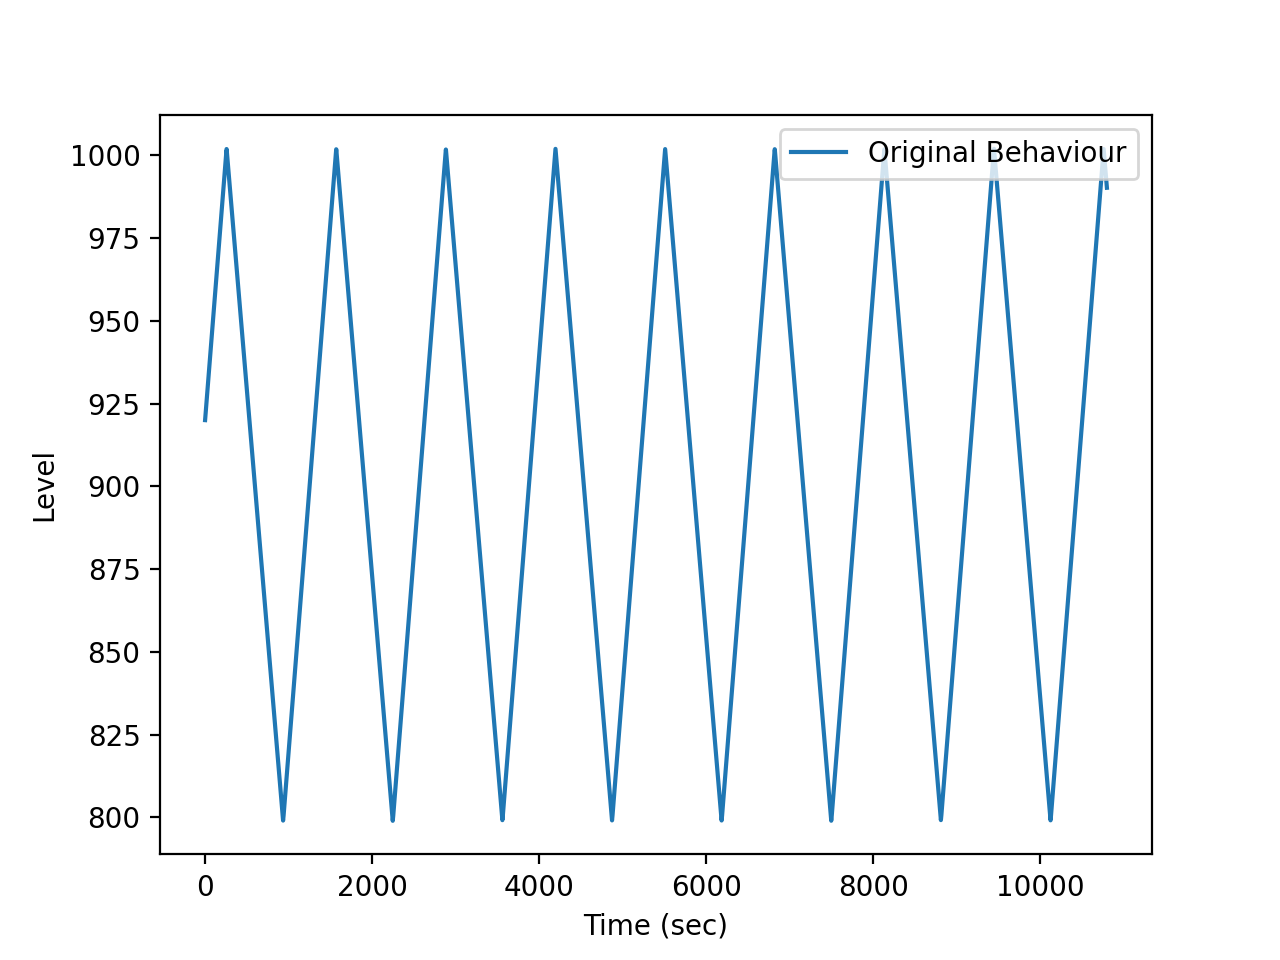
\includegraphics[width=0.4\textwidth]{Figures/Stage3Normal.png}
  \vspace{-0.25cm}
  \caption{Normal steady state behaviour of the water level of Stage 3.}
  \label{fig:Stage3Normal}
  \vspace{-1cm}
\end{wrapfigure}
We establish two simple security requirements for Stage 3: the tank is never empty and the tank never overflows. Formally, these requirements correspond to the invariants $\Always{\vec{x}[L]< 1200}$ and $\Always{\vec{x}[L]> 0}$, defined by

\begin{minipage}{0.5\textwidth}
  \begin{align*}
    \Always{\vec{x}[L]< 1200}&\triangleq \forall k.\vec{x}[L](k)< 1200\\
    \Always{\vec{x}[L]> 0}&\triangleq \forall k.\vec{x}[L](k)> 0.
  \end{align*}
\end{minipage}

Under normal circumstances, the water level of the tank exhibits the behaviour shown in Figure~\ref{fig:Stage3Normal}, so it satisfies the requirements $\Always{\vec{x}[L]< 1200}$ and $\Always{\vec{x}[L]> 0}$.
%\begin{figure}[t]
\subsection*{Testing the Robustness of Stage 3}
Now, consider an attacker model where the attacker can replace at any time the value $\vec{y}[L]$ by any arbitrary value depending on the current real level of water in the tank. 
Under this attacker model, this amounts to a universe of 64 different \emph{representative attacks}, which define when and by what to replace the value of $\vec{y}[L]$. 
We explain how we obtain the size of the attack universe in Section~\ref{sec:AttackerCapabilities}. 

Informally, the robustness of Stage 3 with respect to this attacker model can be measured by the number of attacks that do not break any requirements. Testing shows that 40 out of 64 attacks can break at least one requirement, so the robustness factor of this system is 24/64 with respect to an attacker that controls $\vec{y}[L]$. We explain the process of computing robustness more precisely in Section~\ref{sec:LatentBehaviours}.

\subsection*{Counter-attackers}
So far, we have used a traditional fault-injection to quantify the robustness of Stage 3 with respect to an attacker that controls the sensor $\vec{y}[L]$. 
Now, we rely on the fundamental observation that an attack $m$ on the original version of Stage 3 reveals a latent behaviour, which we denote Stage $3_m$. 
A transformation $w$ on the revealed system Stage $3_m$ may reveal a latent behaviour Stage $3^w_m$ which satisfies all security requirements. 
In such a case, we say that \emph{$w$ is a counter-attack of $m$}.

We now adopt the role of the counter-attacker. Our counter-attacker model allows us to set the values $\vec{q}[P]$ and $\vec{q}[MV]$ in the controller at any time by any arbitrary value we choose; we also assume that we can observe the value $\vec{y}[L]$, which is currently controlled by the original attacker. Under this counter-attacker model, we can define a universe of 729 counter-attacks. We explain how we obtain the size of the counter-attack universe in Section~\ref{sec:CounterAttacks}.

We test counter-attacks on the latent behaviours revealed by successful attacks until we find new behaviours that satisfy all security requirements. For example, consider the attack where...
\todo[inline]{@John: please let me know when the visuals are ready. I can choose one attack, one counterattack and put the results here.}

\subsection*{Latent Robustness}
If we can find a counterattacks for each of the 40 successful attacks in the original model, we say the system has a \emph{latent robustness of 64/64} with respect to the given attacker and counter-attacker models; a score of 24 is given by its original robustness and 40 more if counter-attacks are properly implemented. To effectively implement these counter-attacks, we assume that there is a runtime monitor can detect with high accuracy which attack on $\vec{y}[L]$ is taking place, so that we can react to it accordingly. Choosing the wrong counter-attack can be catastrophic, as it may not only not counter the running attack, it might exacerbate its effects.

\todo[inline]{Connector}

 
\section{Cyber-Physical Systems: Physical Requirements and Attacker Models}
\todo[inline]{Small intro that explains what this section is}
Traditional IT security mechanisms such as authentication and message integrity are insufficient for CPS security. %However, as stated in \cite{CPSAttacksAgainstPCS}, 
The major difference between CPS and IT systems is the interaction with the physical world. We share the view of the authors of \cite{CPSSecVinyl}, who state that CPSs security is {specifically} concerned with attacks that cause some physical impact; i.e., attack that affect the integrity of the physical process.  %Traditional IT security mechanisms (e.g., firewalls, encryption, signatures, etc.) normally do not account for physical parts of the system, making them ineffective when faced against attacks that either target or interact with the physical components of CPSs. In this section, we present an Information Flow (IF) inspired integrity analysis for CPSs which accounts for the physical process.
In this section, we present a framework to quantify the integrity of CPSs. This framework consists of several parts:
\todo[inline]{@Eric: complete when all parts are ready}
\begin{enumerate}
  \item a discrete model for CPSs and their semantics; 
  \item ... 
\end{enumerate}

\subsection{A Discrete Model for CPSs}
Figure \ref{fig:IFCPS} presents an extended version of the \emph{supervisor model} \cite{doi:10.1137/0325013}, which serves as the starting point to define our framework for CPSs. 
\begin{figure}
\centering
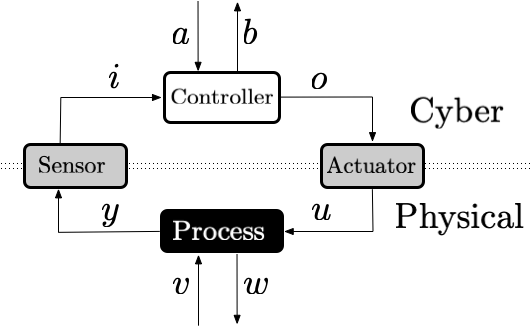
\includegraphics[width=0.45\textwidth]{Figures/IFCPS}
\caption{Extended supervisor model accounting for external inputs and outputs in both cyber and physical components.}
\label{fig:IFCPS}
\end{figure}
Our system model consists of four subsystems: the \emph{controller}, an open, discrete cyber system; the \emph{process}, a linear-time invariant physical system; and two sets of cyber-and-physical interface systems: the \emph{sensors} and the \emph{actuators}. The process, whose state is $\vec{x}$, is observed by the sensor, yielding the physical observation $\vec{y}$; the sensor transforms $\vec{y}$ into the cyber input observation $\vec{i}$. The controller, whose state is $\vec{q}$, receives $\vec{i}$ and an external cyber network input $\vec{a}$, and produces a cyber output network signal $\vec{b}$ and a cyber control signal $\vec{o}$. The cyber signal $\vec{o}$ is then transformed into a physical control signal $\vec{u}$ by the actuator. The process, whose state is $\vec{x}$, reacts to $\vec{u}$ and to some physical network input $\vec{v}$ and yields both a physical network output $\vec{w}$. The then cycle repeats by having the sensor observe the physical state $\vec{x}$ to produce $\vec{y}$. 

Our main objective is to test how well the integrity of the physical state of the process $\vec{x}$ is preserved in the presence of attackers. For this purpose, we define formal notions of \emph{CPS state}, \emph{single-cycle semantics}, and \emph{physical integrity requirements}.
\begin{definition}[States of a CPS]
\label{def:States}
Let us first discuss the role of the non-standard components in our CPS model. The vector of cyber network inputs $\vec{a}$, and the vector of cyber network outputs $\vec{b}$ enable communication between controllers, and play an essential role in CPS composition. The vector of physical network inputs $\vec{v}$, and the vector of physical network outputs $\vec{w}$ model physical channels that connect modules of a larger physical system; e.g. when two water tanks $T_1$ and $T_2$ are connected by a pipe, the outgoing flow from $T_1$ to $T_2$ (a component of $\vec{w}$ for $T_1$) translates to an incoming flow from $T_1$ to $T_2$ (a component of $\vec{v}$ for $T_2$). We use the vector $\vec{i}$ of cyber inputs measurements and the vector $\vec{o}$ of vector of digital control outputs to respectively model communication channels between controller and sensors, and between controller and actuators. Similarly, the vector of physical control inputs $\vec{u}$ and the vector of $\vec{y}$ physical observations model communication channels between the process and actuators, and between the process and sensors. Finally, $\vec{q}$ models the current state of the controller, and $\vec{x}$ models the current state of the process. A \emph{state of the CPS} $\pi$ is the coupling of these vectors; formally, 
\begin{align}
\pi=(\vec{a},\vec{b},\vec{i},\vec{o},\vec{u},\vec{y},\vec{v},\vec{w},\vec{q},\vec{x}).
\end{align}
%$(\vec{a},\vec{b})$ is the state of the network, $(\vec{i},\vec{o},\vec{u},\vec{y})$ is the state of the channels, $(q,x)$ is the \emph{hidden} state of the controller and the process. 
Given a state $\pi$, we denote the value of component $\sigma$ at state $\pi$ by $\pi[\sigma]$. 
%\todo[inline]{@All: for this paper this notation is fine because we do not write things like $\pi[\vec{x}[smt[smt2[smt3]]]]$ or $\pi[\vec{x}][smt][smt2]...$ which is horrible, we write $\pi[\vec{x}[L]]$,though.}

Let $\vec{A}$ be the \emph{range} of $\vec{a}$; i.e., the set of values that $\vec{a}$ can take. Similarly, we define $\vec{B}$, $\vec{I}$, $\vec{O}$, $\vec{U}$, $\vec{Y}$,  $\vec{V}$, $\vec{W}$ $\vec{Q}$, and $\vec{X}$ as the ranges of $\vec{b}$, $\vec{i}$, $\vec{o}$, $\vec{u}$, $\vec{y}$, $\vec{v}$, $\vec{w}$, and $\vec{q}$, respectively. With them we define $\Pi$, the set of all CPS states, by 
\begin{align}
  \Pi\triangleq \vec{A}\times\vec{B}\times\vec{I}\times\vec{O}\times\vec{U}\times\vec{Y}\times\vec{V}\times\vec{W}\times\vec{Q}\times\vec{X}.  
\end{align}
Finally, we informally define the set of \emph{atomic components} $\mathbb{C}$ to be the set of components of states that have no subcomponents. For example, the vector $\vec{u}$ from Section~\ref{sec:example} has two subcomponents, $\vec{u}[MV]$ and $\vec{u}[P]$, so $\vec{u}$ is not an atomic component, but both $\vec{u}[MV]$ and $\vec{u}[P]$ individually are. We refer to the elements of $\mathbb{C}$ as the \emph{coordinates} of the CPS.
\end{definition}

% \begin{minted}{haskell}
% data P1 =
%   P1 {
%     a1::Maybe Bool, -- P2 asking to start/stop inflow of water
%     b1::Maybe Bool, -- P1 informing P2 about the state of p1
%     y1::Float, -- water level in ml
%     ov1::Maybe Bool, -- control signal to v1
%     op1::Maybe Bool, -- control signal to p1
%     p1::Bool, -- physical state of p1
%     v1::Bool, -- physical state of v1
%     t1::Int -- time step
%     } 
% \end{minted}
We now formally define how a state of the CPS evolves over time.
{
\begin{definition}[Single-Cycle Semantics]
\label{def:SingleCycleSemantics}
With $\Pi\triangleq \vec{A}\times\vec{B}\times\vec{I}\times\vec{O}\times\vec{U}\times\vec{Y}\times\vec{V}\times\vec{W}\times\vec{Q}\times\vec{X}$ being the set of states of the CPS, we assume the existence of the following functions,
\begin{itemize}
\item $\delta_{\vec{Q}}\colon \vec{Q}\times \vec{A}\times \vec{I} \rightarrow \vec{Q}$, the transition function of the controller,
%\item $\beta_{\vec{Q}}\colon \vec{Q}\times \vec{A}\times \vec{I} \rightarrow \vec{B}$, the network output function of the controller,
%\item $\theta_{\vec{Q}}\colon \vec{Q}\times \vec{A}\times \vec{I} \rightarrow \vec{O}$, the digital control output function of the controller,
\item $\beta_{\vec{Q}}\colon \vec{Q}\rightarrow \vec{B}$, the network output function of the controller,
\item $\theta_{\vec{Q}}\colon \vec{Q}\rightarrow \vec{O}$, the digital control output function of the controller,
\item $\theta_{\vec{Y}}\colon \vec{Y} \rightarrow \vec{I}$, the translation function of the sensor,
\item $\theta_{\vec{O}}\colon \vec{O} \rightarrow \vec{U}$, the translation function of the actuator,
\item $\delta_{\vec{X}}\colon \vec{X} \times \vec{U}\times \vec{V} \rightarrow \vec{X}$, the transition function of the physical component.
% \item $\beta_{\vec{X}}\colon \vec{X} \times \vec{U}\times \vec{V} \rightarrow \vec{W}$, the physical effect function of the physical component.
%\item $\theta_{\vec{X}}\colon \vec{X}\times \vec{U}\times \vec{V} \rightarrow \vec{Y}$, the physical output function of the process.
\item $\beta_{\vec{X}}\colon \vec{X}\rightarrow \vec{W}$, the physical effect function of the physical component.
\item $\theta_{\vec{X}}\colon \vec{X}\rightarrow \vec{Y}$, the physical output function of the process.
\end{itemize} 
These functions help us control the flow of information; e.g., values of physical variables must go through some sensor to be received by a controller, so a flow from $\vec{x}$ to $\vec{q}$ cannot occur directly. 

We define the single-cycle semantics function $\TheSystem\colon \Pi \rightarrow \Pi$ that describes the evolution of the state $\pi=(\vec{a},\vec{b},\vec{i},\vec{o},\vec{u},\vec{y},\vec{v},\vec{w},\vec{q},\vec{x})$ of the CPS by
\begin{align}
\TheBehaviourOf{\pi}&\triangleq\left((\vec{a'},\vec{b'},\vec{i'},\vec{o'},\vec{u'},\vec{y'},\vec{v'},\vec{w'},\vec{q'},\vec{x'})\right), 
\end{align}
where $\vec{a'}$ and $\vec{v'}$ are external inputs, and 
\begin{gather*}
%\vec{o'}=\theta_{\vec{Q}}(\vec{q},\vec{a},\vec{i}),\quad 
\vec{o'}=\theta_{\vec{Q}}(\vec{q}),\quad 
\vec{q'}=\delta_{\vec{Q}}(\vec{q},\vec{a},\vec{i}),\quad 
%\vec{b'}=\beta_{\vec{Q}}(\vec{q},\vec{a},\vec{i}),\\
\vec{b'}=\beta_{\vec{Q}}(\vec{q}),\\
\vec{x'}=\delta_{\vec{X}}(\vec{x},\vec{u},\vec{v}),\quad
%\vec{y'}=\theta_{\vec{X}}(\vec{x},\vec{u},\vec{v}),\quad \vec{w'}
\vec{y'}=\theta_{\vec{X}}(\vec{x}),\quad 
%\vec{w'}=\beta_{\vec{X}}(\vec{x},\vec{u},\vec{v}),\\
\vec{w'}=\beta_{\vec{X}}(\vec{x}),\\
\vec{u'}= \theta_{\vec{O}}(o),\quad\vec{i'}=\theta_{\vec{Y}}(\vec{y}).
\end{gather*}
%i.e. for all $k$, $\vec{i}(k)=\vec{y}(k)$ and $\vec{u}(k)=\vec{o}(k)$. 
The evolution over $k+1$ cycles is defined by iterating $\TheSystem$, \emph{i.e.},
\begin{align}\label{eq:kCycles}
\TheSystem_{k+1}&= \TheSystem \circ \TheSystem_{k}.
\end{align}
Finally, we define $\TheBehaviourOf{\pi}_{0}=\pi$ for all states $\pi \in \Pi$. Under this definition, the \emph{normal behaviour} of the CPS is characterised by the infinite sequences $(\pi_0, \pi_1, \ldots)$ where $\pi_{k+1}\triangleq\TheBehaviourOf{\pi_k}$ and $\pi_0$ is an initial state.%; equivalently $\pi_{k}\triangleq \TheBehaviourOf{\pi_0}_k$.
\end{definition}
}
Because a CPS itself does not create values for $\vec{a}$ and $\vec{v}$, we need a stream of network inputs $(\vec{a_0}, \vec{a_1}, \ldots)$ and a stream of physical effects $(\vec{v_0}, \vec{v_1}, \ldots)$ to advance the system. Usually, $\vec{a}$ is given by another CPS as a function of the network output $\vec{b}$ of the latter CPS; similarly, $\vec{v}$ is given as a function of the physical output $\vec{w}$ from another system. If the functions $\delta_{\vec{Q}}$ and $\delta{\vec{X}}$ respectively ignore $\vec{a}$ and $\vec{v}$ for their computation, then we say that the CPS is \emph{closed}.
Henceforth, we assume that the CPS (or composition of CPSs) we are working with is closed. We show an example of a CPS composition in Section~\ref{sec:CaseStudy}.

In the following, we define a notion of integrity based on security requirements over physical components, the attacker models we consider in this work, a method to systematically generate attacks, and a method to model the attackers that can execute them. 

\subsection{Physical Requirements}{
{\color{blue}
\todo[inline]{@All: this section in blue remains from the workshop version. We could keep it, unless you feel it does not fit the tone of the paper.}
Clarkson and Schneider state in \cite{QuantitativeIntegrity} that they know of no widely accepted definition of integrity, but they remark that an ``informal definition seems to be the `prevention unauthorized modification of information'." Clarkson and Schneider use two formal notions to characterise and quantify the {damage to integrity}, which they refer to as \emph{corruption} of information. One notion is \emph{contamination}, a generalisation of taint analysis that tracks information flows from untrusted inputs to outputs that are supposed to be trusted. The other notion is \emph{suppression}, which occurs when implementation outputs omit information about correct outputs (with respect to the specification). Contamination is dual to information leakage under the Biba duality; however, there is no apparent Biba dual to suppression \cite{BibaIntegrity}. 
}
%Both contamination and suppression are present in CPSs. For example physical attackers can contaminate the state of physical components by directly interacting with them (e.g. an attacker jamming a pump), and cyber attackers can suppress the communication between controllers (e.g. by launching a mitm attack).
In this work, we want to test whether any corruption generated either by contamination or by suppression of information affects the integrity of the behaviour of the system. To that end, we %want to minimise the restrictions we impose over attackers; more precisely, we believe 
give attackers the ability to arbitrarily contaminate (e.g. by linearly transforming the real value) or suppress (e.g., by arbitrary substitution of the real value) the information in the components they can directly interact with, while only abiding to a minimal type-checking restriction: the input provided by the attacker must have the same type as the corrupted input, or the behaviour of the system becomes ill-defined. Moreover, we allow attackers to have some view over the current state of the system, so they can decide when and how to corrupt the system.

%\todo[inline]{Ultimately, it does not matter whether the attacker wants to reuse the current value in some way(contaminate), or set a fixed value (suppress), because only some values matter, and they only matter under certain conditions.}
%\todo[inline]{This discussion on information flow should be very vague, considering that we do not really use entropy or anything else related to information flow. It makes for an interesting introduction though; we should just be careful that the readers don't get the wrong idea.} 

Before we formally define attackers and their attacks, we introduce the notion of \emph{physical (integrity) requirement}. We use physical requirements to determine when the behaviour of the process $\vec{x}$ has deviated critically, and becomes unsafe. Formally, physical requirements model safety properties over the physical state.
\begin{definition}[Physical Requirement]
  Let $\Pi$ be the set of states of the CPS. A \emph{physical requirement} is a finite state automaton $\TheRequirement=(S,\delta,F,s_0)$, where $S$ is a set, $\delta\colon S\times \vec{X}\rightarrow S$ is the transition function, $F\subseteq S$ marks critical states, and $s_0\in S$ is the initial state. Given a possibly infinite sequence of states of the CPS $\omega=(\pi_0,\pi_1 \ldots)$, we say that \emph{$\omega$ breaks the physical requirement modelled by $\mathbb{R}$} if and only if there exists a finite prefix of $\omega$, say $(\pi_0,\ldots\pi_n)$, such that the sequence $(\pi_0[\vec{x}],\ldots, \pi_n[\vec{x}])$ is rejected by $\TheRequirement$.
\end{definition}
%\todo[inline]{Awesome! now we can model a requirement that states that the water level of the tank must not remain low for large periods of time, or the pump would burn.}
We expect the original CPS to satisfy all physical requirements. More precisely, since the normal behaviour of the CPS are the sequences $(\pi_0, \pi_1, \ldots)$ where $\pi_{k+1}=\TheBehaviourOf{\pi_k}$ and $\pi_0$ is an initial state, we expect, for all $k$, that the sequences $(\pi_0[\vec{x}],\ldots,\pi_k[\vec{x}])$ is accepted by every physical requirement.

\subsection{Attacks as Vector Fields on the Phase Space}
Now that we have a behaviour function that maps states to states, i.e., the single cycle semantics function $\TheSystem\colon\Pi\rightarrow\Pi$ from Definition~\ref{def:SingleCycleSemantics}, we can compose it with an arbitrary state transformation $m\colon \Pi\rightarrow\Pi$ to reveal a new behaviour function $\TheSystem\circ m\colon\Pi\rightarrow\Pi$, which may or may not satisfy the physical requirements.

% In Section~\ref{sec:example} we hinted the possibility of describing attacks as vectors. In this section, we discuss in more detail the meaning of the bases and the coefficients of attacks.
To describe an attack $m\colon \Pi\rightarrow \Pi$ as a vector, we need a basis and a set of coefficients. The basis reflects the visibility of the attacker over the current state of the system, so it also characterises the ability of the attacker to estimate when the current state of the system satisfies a relevant condition. The most granular base is given by the elements of $\Pi$ (when $\Pi$ is finite), and it models an attacker with absolute visibility; i.e. the attacker always knows the value of every component of the current state. The least granular base is given by $\Pi$ itself, and it models an attacker with no visibility over the current state.
\begin{definition}[Attack Basis]
  \label{def:AttackBasis}
Let $\Pi$ be the set of states of the CPS. An \emph{attack basis} is any \emph{finite} partition $\sum_{i=1}^n \Pi_i$ of $\Pi$ such that, for $1\leq i,j \leq n$ the following conditions hold: $\Pi_i$ is non-empty, every $\Pi_i$ is disjoint from every other $\Pi_j$ in the partition, and the union of all $\Pi_i$ is $\Pi$. We often refer to an element of the partition $\Pi_i$ by its characteristic predicate.
\end{definition}
\begin{example}
  \label{ex:AttackBasis}
  For Stage 3 from Section~\ref{sec:example}, we define the base $[LL, OK, HH]^T$, where ${LL}=\set{\pi| \pi[\vec{x}[L]]<Lmin}$, ${HH}=\set{\pi| \pi[\vec{x}[L]]>Lmax}$ and ${OK}=\set{\pi|Lmin \leq \pi[\vec{x}[L]]\leq Lmax}$. The base $[LL, OK, HH]^T$ models the visibility of an attacker that can always determine whether the current state of the system is in $LL$, in $OK$ or in $HH$.  %We refer to $\set{\pi\in \Pi| \pi[\vec{x}[L]]>Lmax}$ by $(\vec{x}[L]>Lmax)$ and we refer to $\Pi$ by $\True$.
\end{example}

The coefficients of an attack vector model the capabilities of the attacker to interact with the system. The natural choice for this set of coefficients is the monoid $(\Pi\rightarrow \Pi, \circ, \id)$, because it enables attack composition. However, since we are interested in creating a test suite to systematically test latent behaviours, we want a finite set of \emph{representative coefficients} that spans a finite number of attacks. Thus, we generate an {idempotent monoid} using constant transformations of coordinates.%, henceforth named $\IMCT$.

% \begin{definition}[\textbf{I}dempotent \textbf{M}onoid Generated by \textbf{C}onstant \textbf{T}ransformations in one atomic component (\textbf{$\IMCT$})]
\begin{definition}[Idempotent Monoid Generated by Constant Transformations of Coordinates {$\IM{\Gamma_{\mathcal{K}}}$}]
  \label{def:IdempotentMonoid}
We define the \emph{constant transformation of the atomic component $c$ to value $v$}, denoted $\const^{c}_{v}\colon \Pi\rightarrow \Pi$, for all $\pi \in \Pi$ and $c'\in \mathbb{C}$ by
  \begin{align}
    \const^{c}_{v}(\pi)[c']& \triangleq 
    \begin{cases}
     v, &\quad \text{if $c'=c$,}\\
     \pi[c']&\quad \text{otherwise.}
    \end{cases}
  \end{align} 
Let $\Gamma_\mathcal{K}$ be a \emph{finite} set of constant transformations of coordinates from a set $\mathcal{K}\subseteq\mathbb{C}$. Each $\const^{c}_{v}\in \Gamma_\mathcal{K}$ characterises a \emph{representative value} $v$ of $c$.
% generated from a finite set of \emph{representative values}. More precisely, let $\vec{C}$ be the range of $c$; given some representative value $v\in \vec{C}$, there exists a transformation $\const^{c}_{v}\in \Gamma_c$.

% Now, each atomic component $c$ defines a set of generators $\const(\Gamma_c)$, formally defined by
% \begin{align}
%   \const(\Gamma_c)\triangleq \set{\const^{c}_{v} | v\in\Gamma_c}.
% \end{align}
We generate the monoid $(\IM{\Gamma_{\mathcal{K}}},\circ,\id)$ %by choosing $\mathcal{K}=\mathbb{C}$, and 
by closing %the union of all $\Gamma_c$ in the family $\Gamma_{\mathbb{C}}$ 
$\Gamma_{\mathcal{K}}$ under function composition; the unit of the monoid is the identity function $\id$, and the operation is function composition $\circ$. 

%$\AsSequence{\ucup_{c\in \mathbb{C}}\const(\Gamma_c)}$
% \begin{definition}[Single Component Transformations]
% Let $c\colon \Pi\rightarrow \Pi$. We say that $c$ is a \emph{single-component transformation (on $\sigma$)} of the elements of $\Pi$ if and only if $c=\id$, or there exists one and only one component $\sigma$ such that 
% \begin{align}
%   c(\pi)[\sigma]=\pi[\sigma],
% \end{align} 
% and $\sigma$ has no subcomponents. 
%Due to properties of the monoid and because 
Since each transformation $t\in \IMCT$ is finitely generated, $t$ unambiguously pairs each atomic component $c\in \mathbb{C}$ with either $\id$ or with some constant transformation $\const^{c}_{v}$ in $\Gamma_{\mathcal{K}}$.  We denote this association by $t[c]$. If $t[c]=\id$, then $t$ does not act on the atomic component $c$, and if $t[c]=\const^{c}_{v}$, then $t(\pi)[c]=v$ for all $\pi \in \Pi$.
\end{definition}
\begin{example}
  In the context of Stage 3 from Section~\ref{sec:example}, an attacker can infer from Equation~\ref{eq:ControllerStager3} that, if $\vec{y}[L](k)\geq Lmax$% and $\vec{q}[MV](k)=\texttt{open}$
  , then $\vec{u}[MV](k+1)$ is $\texttt{closing}$. From this knowledge, if the attacker aims to keep the valve $MV$ closed by attacking $\vec{y}$, then they should transform $\vec{y}$ into a value $\bar{y}$ that satisfies $\bar{y}[L](k)\leq Lmax$; similarly, if they aim to keep $MV$ open, then $\bar{y}$ should satisfy $\bar{y}[L](k)\leq Lmin$. The concrete values of $\bar{y}[L](k)$ are unimportant as long as they satisfy the desired condition. In that sense,the attacker chooses the \emph{representative values} $500~\mathrm{L}$, $800~\mathrm{L}$ and $1100~\mathrm{L}$ for $\bar{y}[L](k)$. These representative values characterise the set of constant transformations $\Gamma_{\vec{y}[L]}$, given by
\begin{align}
  \Gamma_{\vec{y}[L]}=\set{\const_{500}, \const_{800},  \const_{1100}}.
\end{align}
If we close the set $\Gamma_{\vec{y}[L]}$ under function composition, and we include the $\id$ transformation, we obtain the idempotent monoid $\IM{\Gamma_{\vec{y}[L]}}$, where 
\begin{align*}
  \IM{\Gamma_{\vec{y}[L]}} =\set{\id, \const_{500}, \const_{800},\const_{1100}}.
\end{align*} 
\end{example}

We finally define attacks by combining coefficients from $\IMCT$ and a basis $\sum\Pi$.
\begin{definition}[Attack]
  \label{def:Attack}
Given a basis $\sum_{i=1}^n\Pi_i$ and coefficients $t_1, \ldots, t_n\in\IMCT$, 
 %generated by the representative values $\Gamma_c$ for each $c\in \mathbb{C}$, 
we define an \emph{attack} $\vec{m}\colon \Pi\rightarrow \Pi$, for $\pi\in \Pi$, with the linear combination
\begin{align}
  \vec{m}=t_1\Pi_1 + t_2\Pi_2 + \ldots + t_n\Pi_n,
\end{align} 
or, equivalently, with the function
\begin{align}
  \label{eq:AttackVector}
  \vec{m}(\pi)=
    \begin{cases}
      t_1(\pi), &\quad\text{if $\pi\in \Pi_1$;}\\
      \ldots&\quad\ldots\\
      t_n(\pi), &\quad\text{if $\pi\in \Pi_n$.}
    \end{cases}
\end{align}
For convenience, we write $\vec{m}$ using vectors as follows: 
\begin{align}
  \vec{m}(\pi)=
  %[t_1,\ldots,t_n]
  \begin{bmatrix}
    t_{1} \\
    \vdots \\
    t_{n}
  \end{bmatrix}
  \cdot
  \begin{bmatrix}
    \Pi_{1} \\
    \vdots \\
    \Pi_{n}
  \end{bmatrix}.
\end{align} 
We can scale an attack $\vec{m}\colon \Pi\rightarrow \Pi$ by $t\in \IMCT$ to obtain the attack $t\vec{m}\colon \Pi\rightarrow \Pi$, defined for $\pi\in \Pi$ by
\begin{align}
  t\vec{m}(\pi)\triangleq
  %[t_1,\ldots,t_n]
  \begin{bmatrix}
    t\circ t_{1} \\
    \vdots \\
    t\circ t_{n}
  \end{bmatrix}
  \cdot
  \begin{bmatrix}
    \Pi_{1} \\
    \vdots \\
    \Pi_{n}
  \end{bmatrix}.
\end{align} 
We can also add attacks using function composition, which is \emph{not commutative}. Composition of attacks using the same basis corresponds to composing their coefficients. However, composing attacks with different bases requires a common basis. Given attacks $\vec{m}_1$ and $\vec{m}_2$ whose respective bases are $\sum_{i=1}^n\Pi_i$ and $\sum_{i=1}^m\Pi'_i$, 
we define the common basis $(\sum_{i=1}^n\Pi_i)(\sum_{i=1}^m\Pi'_i)$ by 
\begin{align}
  \left(\sum_{i=1}^m\Pi'_i\right)\left(\sum_{i=1}^n\Pi_i\right)\triangleq \sum_{j=1}^m\sum_{i=1}^n(\Pi'_j\cap\Pi_i);
\end{align}
% To compose $\vec{m}_1$ and $\vec{m}_2$ it is convenient to express them as linear combinations as follows

% \begin{align*}
%   \vec{m}_2\circ \vec{m}_1&=(t'_1\Pi'_1 + \ldots + t'_m\Pi'_m)(t_1\Pi_1 + \ldots + t_n\Pi_n)\\
%   &=t'_1\Pi'_1(t_1\Pi_1 + \ldots + t_n\Pi_n)+ \ldots t'_m\Pi'_m(t_1\Pi_1 + \ldots + t_n\Pi_n)\\
%   &=(t'_1\circ t_1)(\Pi'_1\cap\Pi_1) + \ldots (t'_1\circ t_n)(\Pi'_1\cap\Pi_n)+ \ldots \\
%   &+(t'_m\circ t_1)(\Pi'_m\cap\Pi_1) + \ldots + (t'_m\circ t_n)(\Pi'_m\cap\Pi_n).
% \end{align*} 
%in its vectorial form it corresponds to
so the sum of $\vec{m}_2$ and $\vec{m}_1$ then is defined by
\begin{align}
  (\vec{m}_2+\vec{m}_1)(\pi)=(\vec{m}_2\circ\vec{m}_1)(\pi)\triangleq
  %[t_1,\ldots,t_n]
  \begin{bmatrix}
    t'_{1}\circ t_1 \\
    \vdots \\
    t'_{1}\circ t_n\\
    \vdots \\
    t'_{m}\circ t_1 \\
    \vdots \\
    t'_{m}\circ t_n
  \end{bmatrix}
  \cdot
  \begin{bmatrix}
    \Pi'_{1}\cap\Pi_{1} \\
    \vdots \\
    \Pi'_{1}\cap\Pi_{n}\\
    \vdots \\
    \Pi'_{m}\cap\Pi_{1} \\
    \vdots \\
    \Pi'_{m}\cap\Pi_{n}\\
  \end{bmatrix}.
\end{align} 
Finally, if the states of the CPS must satisfy a physical invariant $\mathcal{I}\colon \vec{x}\rightarrow\bool$, then we say that an attack $m$ is \emph{physically impossible} if there exists some state $\pi\in \Pi$ such that $\pi[\vec{x}]$ satisfies $\mathcal{I}$, but $\vec{m}(\pi)[\vec{x}]$ does not.
\todo[inline]{Physical invariants may go beyond $\vec{x}$, but I'll just keep them restricted to $\vec{x}$ for now.}
\end{definition}

\begin{example}
  \label{ex:attack}
  In the case of Stage 3 from Section~\ref{sec:example}, we define an attack $m$ using the basis $[LL, OK, HH]^T$ and the coefficients $\Gamma_{\vec{y}[L]}=\set{\const_{500}, \const_{800},  \const_{1100}}$, by
\begin{align}
  \vec{m}=
  \begin{bmatrix}
    \id \\
    \const_{500} \\
    \const_{500}
  \end{bmatrix}
  % [\id,\const_{500},\const_{500}]
  \cdot
  \begin{bmatrix}
    LL \\
    OK\\
    HH
  \end{bmatrix}.
\end{align}
The transformation $m$ describes an attack where the attacker forces the value of $\vec{y}[L]$ to be $500$, but only when the current state satisfies either $OK$ or $HH$; otherwise, it keeps the current value. This attack causes the tank to overflow after about 876 cycles.
\end{example}
The $\IMCT$ captures the capabilities of attackers in two ways. First, the $\IMCT$ explicitly models that each attacker to only tries a set of representative values that they deem interesting when attacking a component $c$, since they expect these values to trigger different behaviours in the system. Second, the $\IMCT$ characterises the minimal set of components that must be under the control of the attacker so that attacks are possible; i.e. the \emph{required attacker capabilities}.

\subsection{Attacker Capabilities}
\label{sec:AttackerCapabilities}
In general, we relate the \emph{capabilities} required to execute an attack $m$ to the set of changes in atomic components that the attacker needs to perform to apply the attack $m$ in every state of the CPS.  %Informally, the Hamming distance between two states $\pi_1$ and $\pi_2$ denotes the minimum set of coordinates that must be changed to turn $\pi_1$ into $\pi_2$ or vice versa. 
\begin{definition}[Required Capabilities]
Let ${m}\colon \Pi\rightarrow \Pi$; we define the \emph{capabilities required to execute $m$}, denoted $|m|$, to be the set  
\begin{align}
  %|m|\triangleq \set{c \in \mathbb{C}| \pi[c]\neq m(\pi)[c],\text{ for some $\pi\in\Pi$.}}
  |m|\triangleq \left\{\const^c_{m(\pi)[c]}\ |\ \pi[c]\neq m(\pi)[c],\text{ for $\pi\in\Pi$ and $c\in \mathbb{C}$.}\right\}
\end{align}
\end{definition}
In general, computing the required capabilities of an arbitrary given transformation $m\colon \Pi\rightarrow\Pi$ requires us to apply $m$ to all elements in $\Pi$, and then check which components did not change. However, by using the $\IMCT$, we can compute the {capabilities} required to execute an attack directly from their definition, as shown in the following Corollaries~\ref{cor:Capabilities} and \ref{cor:GeneralCapabilities}. 

\begin{corollary}
\label{cor:Capabilities}
Since every $t\in \IMCT$ pairs each component $c$ in $\mathbb{C}$ to some $\const^{c}_{v}$ or to $\id$, 
%is finitely generated by a composition of constant transformations of $n$ different atomic components, i.e., $t= \const^{c_n}_{v_n}\circ \ldots \circ \const^{c_1}_{v_1}$, 
the set of required capabilities to execute $t$ is 
\begin{align}
  |t|=\set{t[c]| t[c]\neq \id \text{ and } t[c]=\const^{c}_{v}, \text{for $c\in \mathbb{C}$}}.
  %\const^{c_1}_{v_1},\ldots, \const^{c_n}_{v_n}}
\end{align}
\end{corollary}
%Corollary~\ref{cor:Capabilities} implicitly states that we can construct an attacker model by looking at the definition attack. 
\begin{corollary}
  \label{cor:GeneralCapabilities}
If $\vec{m}=[t_1\ldots + t_n]^T\cdot[\Pi_1, \ldots, \Pi_n]^T$, then the set of capabilities required for the attack $\vec{m}$ is the union of the capabilities required for its coefficients. Formally, 
\begin{align}
  |\vec{m}|=\bigcup_{i=1}^n|t_i|.
\end{align}
\end{corollary}
% \todo[inline]{@All: this is the reason why we actually bothered to define the $\IMCT$. It lets us both generate attacks from an attacker model, and also construct an attacker model from a given attack.}

We associate attacks to some \emph{attacker model}.
%and we want attacker models to define universes of attacks. 
Informally, an attacker model defines a set of capabilities given to attackers to conduct their attacks, and describes the universe of attacks available to attackers that fit the model. 
\begin{definition}[Attacker Model]
 Let $\Gamma_\mathcal{K}$ be a set of constant transformations of coordinates $c$ in some $\mathcal{K}\subseteq\mathbb{C}$, and let $\sum_{i=1}^n\Pi_i$ be a basis; the pair $\mathcal{A}=(\Gamma_{\mathcal{K}}, \sum_{i=1}^n\Pi_i)$ defines the \emph{attacker model} that characterises attackers that have visibility $\sum_{i=1}^n\Pi_i$ over the CPS and that are capable of applying the transformations in $\IM{\Gamma_\mathcal{K}}$ %\subseteq \IM{\Gamma_\mathbb{C}}$ 
  to the states of the CPS, \emph{but only those transformations}. %Any transformations that are not in the submonoid $\IM{\Gamma_\mathcal{K}}$ are beyond the capabilities of attacker that fit this model.%, \emph{but only those}.
  
  The attacks characterised by the attacker model $(\Gamma_{\mathcal{K}}, \sum_{i=1}^n\Pi_i)$ are the vectors whose coefficients are elements of $\IM{\Gamma_\mathcal{K}}$ and whose basis is $\sum_{i=1}^n\Pi_i$. Dually, we associate each attack $\vec{m}$ using some base $\sum_{i=1}^n\Pi_i$ with the attacker model whose capabilities are barely enough to execute $\vec{m}$; i.e., the \emph{free attacker model of $\vec{m}$}, which is $(|\vec{m}|, \sum_{i=1}^n\Pi_i)$.
  % The attacks associated to the attacker model  be the idempotent submonoid of constant transformations on atomic components constructed following Definition~\ref{def:IMCT} using $\mathcal{C}$ and $\Gamma_{C}$,is generated using the components defines an \emph{attacker model} . 
\end{definition}
%\todo[inline]{@Eric: maybe parametrise the $\IMCT$ in its definition??}
\begin{example}
  In general, the pair $(\Gamma_{\emptyset}, \Pi)$ models a passive attacker, since the only attack of this model is $\vec{id}=[\id]\cdot[\True]$; i.e. an attack that does not change the state. %, since $\id$ is the only element of the monoid $\IM{\Gamma_{\emptyset}}$. 

  Now, consider the attacker model $(\Gamma_{\vec{y}[L]},\set{LL,OK,HH})$ in the context of Stage 3 of Section~\ref{sec:example}. This attacker model describes attacks that can affect $\vec{y}[L]$ differently depending on whether the state satisfies $LL$, $OK$ or $HH$; 
  however, their effects over $\vec{y}[L]$ are limited to $\IM{\Gamma_{\vec{y}[L]}}=\left\{\id, \const^{\vec{y}[L]}_{500}, \const^{\vec{y}[L]}_{800}, \const^{\vec{y}[L]}_{1100}\right\}$. This attacker model consists of 64 different attacks, given by the combination ${\left|\IM{\Gamma_{\vec{y}[L]}}\right|}^{\left|\set{LL,OK,HH}\right|}=4^3$
\end{example}

% , where $\Gamma_{|\vec{m}|$ is the family of functions 
% \begin{align}
%   \Gamma_{|\vec{m}|}\triangleq\bigcup_{i=1}^n |t_i|.
% \end{align}

Now that we have a method to systematically generate attacks and to associate them with an attacker model, we are ready to use them to reveal latent behaviours. 

% \begin{definition}[Hamming distance]
% Let $\mathbb{C}$ be the set of coordinates of the CPS. Given states $\pi_1$ and $\pi_2$ in $\Pi$, we define the hamming distance between $\pi_1$ and $\pi_2$, denoted $|\pi_1-\pi_2|$, by the set
% \begin{align}
%   |\pi_1-\pi_2|\triangleq \set{c \in \mathbb{C}| \pi_1[c]\neq \pi_2[c]}.
% \end{align}
% \end{definition}
\section{Testing and Improving Robustness via Latent Behaviour Analysis}
\label{sec:LatentBehaviours}
The robustness of a system is a measure relative to some attacker model. The more attacks there are, and the more the system resists them without failing its requirements, the more robust it is. In this section, we formally define a notion of robustness for a CPS with respect to a given attacker model, and we show how to improve it with respect to a given counter-attacker model.

An attack $\vec{m}$ continuously changes the state of the system, altering its single-cycle semantics and revealing a \emph{latent behaviour}. More precisely, we can compose the single-cycle semantics $\TheSystem$ with an arbitrary state transformation $m\colon \Pi\rightarrow\Pi$ to reveal a new behaviour function $\TheSystem\circ m\colon\Pi\rightarrow\Pi$. We call $\TheSystem\circ m$ the \emph{latent behaviour} revealed by $m$, because it depends on the latent/hidden variable $m$. 

\begin{definition}[Latent Behaviour]
  \label{def:LatentBehaviour}
  Given an attack $\vec{m}\colon \Pi\rightarrow \Pi$, the \emph{latent behaviour revealed by $\vec{m}$} at some initial state $\pi_0$ is the (infinite) sequence of states $(\pi^{\vec{m}}_0, \pi^{\vec{m}}_1\ldots)$ inductively defined, for $k\geq 0$, by 
  \begin{align}
    \label{eq:newkCycle}
    %\TheSystem^m&\triangleq\TheSystem \circ m\\
    {\pi}^{\vec{m}}_{k+1}\triangleq \TheBehaviourOf{\vec{m}({\pi}^{\vec{m}}_{k})}, \quad \text{with ${\pi^{\vec{m}}_{0}}\triangleq \pi_0$.}
    %\TheSystem^m &\triangleq \TheSystem \circ m\quad\text{and}\quad 
  \end{align}
% \begin{align}
% \TheSystem^m_{k+1}&\triangleq (\TheSystem \circ m) \circ\TheSystem^{m}_{k}, \quad \text{with $\TheSystem^m_{0}=m$.}
% \end{align}
In the following, we slightly abuse notation and refer to the latent behaviour $(\pi^{\vec{m}}_0, \pi^{\vec{m}}_1\ldots)$ by $\TheSystem^{\vec{m}}$.
\end{definition}
Given an attacker model $\mathcal{A}$, and a set of requirements $\TheSetOfRequirements$, we define the \emph{robustness} of the system to be the number of attacks that fail to break any physical requirement over the total number of attacks generated by the attacker model.

% In this section, we show how to model attacks as these transformations $m$ to reveal a latent behaviour of the system under attack $\TheSystem\circ m$. We can then use the revealed latent behaviours $\TheSystem\circ m$ to quantify robustness via testing, which we do in Section~\ref{sec:LatentBehaviours}.
\begin{definition}[Robustness]
  Given an attacker model $\mathcal{A}$, and a set of requirements $\TheSetOfRequirements$, we define $\mathcal{A}(\TheSetOfRequirements)$ to be the set of attacks in $\mathcal{A}$ that break at least one requirement. We define 
  the \emph{robustness} of the system by 
  \begin{align*}
    \frac{|\mathcal{A}|-|\mathcal{A}(\TheSetOfRequirements)|}{|\mathcal{A}|}
  \end{align*}
\end{definition}

\begin{example}
  In the context of the attacker model of Stage 3 where the basis is $[LL, OK, HH]^T$ and the coefficients are $\Gamma_{\vec{y}[L]}=\set{\const_{500}, \const_{800},  \const_{1100}}$, there are 64 attacks, out of which 40 break at least one physical requirement. The robustness of Stage 3 with respect to this attacker model is 24/64.
\end{example}
%\todo[inline]{@All: can someone please edit the following sections? I'm writing extremelly informally}
\subsection{Counter-Attacks and Latent Robustness}
\label{sec:CounterAttacks}
Latent behaviour analysis teaches us that attacks transform the single-cycle semantics, so it is possible for us to keep transforming the revealed latent behaviours with other transformations: \emph{counter-attacks}. Counter-attacks are exactly the same as attacks, but we use them to reveal second-degree latent behaviours; i.e. the latent behaviours of the latent behaviours revealed by attacks on the original system. 

% \begin{definition}[Counter-Attack]
%   \label{def:CounterAttack}
% Given a basis $\sum_{i=1}^n\Pi_i$ and coefficients $t_1, \ldots, t_n\in\IMCT$, 
%  %generated by the representative values $\Gamma_c$ for each $c\in \mathbb{C}$, 
% we define a \emph{counter-attack} $\vec{w}\colon \Pi\rightarrow \Pi$, for $\pi\in \Pi$, with the linear combination
% \begin{align}
%   \vec{w}=t_1\Pi_1 + t_2\Pi_2 + \ldots + t_n\Pi_n.
% \end{align} 
% For convenience, we write $\vec{w}$ using vectors as follows, 
% \begin{align}
%   \vec{m}(\pi)=
%   %[t_1,\ldots,t_n]
%   \begin{bmatrix}
%     t_{1} \\
%     \vdots \\
%     t_{n}
%   \end{bmatrix}
%   \cdot
%   \begin{bmatrix}
%     \Pi_{1} \\
%     \vdots \\
%     \Pi_{n}
%   \end{bmatrix}.
% \end{align} 
% \end{definition}

A \emph{counter-attacker models} are dual to attacker models. Given that the controller or the operator would play the role of the counter-attacker, we can give them extraordinary privileges. More precisely, we believe it is sensible to describe the counter-attacker model as a rather capable attacker whose transformations directly affect the controller or the physical components the system. 

\begin{example}
  \label{ex:counterattack}
  In the context of Stage 3 from Section~\ref{sec:example}, we define the counter-attacker model $(\Gamma_{\set{\vec{q}[MV],\vec{q}[P]}},\set{\widehat{LL},\widehat{OK},\widehat{HH}})$. The idempotent monoid of coefficients is generated by $\Gamma_{\vec{q}[MV],\vec{q}[P]}$, where 
  \begin{align*}
    \Gamma_{\set{\vec{q}[MV],\vec{q}[P]}}&=\Gamma_{\vec{q}[MV]}\cup\Gamma_{\vec{q}[P]}\\
    &=\set{\const^{\vec{q}[MV]}_{\texttt{open}},\const^{\vec{q}[MV]}_{\texttt{closed}}}\\
    &\cup \set{\const^{\vec{q}[P]}_{\texttt{on}},\const^{\vec{q}[P]}_{\texttt{off}}}
  \end{align*}
  The basis $\set{\widehat{LL},\widehat{OK},\widehat{HH}}$ is defined by  $\widehat{LL}(\pi)=(\pi[\vec{y}[L]]<Lmin)$, $\widehat{HH}(\pi)=(\pi[\vec{y}[L]]>Lmax)$ and $\widehat{OK}(\pi)=(Lmin\leq \pi[\vec{y}[L]]\leq Lmax)$. Note that we arbitrarily choose the visibility of the counter-attacker to be affected by the attacker. More precisely, we use $\widehat{LL},\widehat{OK}$ and $\widehat{HH}$, which depend on the level provided by the attacker $\vec{y}[L]$, and not on the physical (real) water level $\vec{x}[L]$. 
  % (Y[L3]<L3min)=>[(Q[MV3]->closed), (Q[P3]->off)] + (L3min<=Y[L3]<=L3max)=>[id(Q[MV3]), id(Q[P3])] + (Y[L3]>L3max)=>[id(Q[MV3]), id(Q[P3])]
  This counter-attacker model generates 729 different counter-attacks, 
since
\begin{align*}
  \left| \IM{\Gamma_{\set{\vec{q}[MV],\vec{q}[P]}}}\right|^{\left|\set{\widehat{LL},\widehat{OK},\widehat{HH}}\right|}=9^3=729
\end{align*}
  An example counter-attack $\vec{w}$ from this model is 
  \begin{align}
    \vec{w}=
    \begin{bmatrix}
      \const^{\vec{x}[MV]}_{\texttt{closed}} \circ \const^{\vec{x}[P]}_{\texttt{off}} \\
      \id \\
      \id
    \end{bmatrix}
    % [\id,\const_{500},\const_{500}]
    \cdot
    \begin{bmatrix}
      \widehat{LL} \\
      \widehat{OK}\\
      \widehat{HH}
    \end{bmatrix}.
  \end{align}
\end{example}

\begin{definition}[Attack Countering]
  We say that a counter-attack $\vec{w}$ \emph{counters} an attack $\vec{m}$ if and only if the latent behaviour $\TheSystem\circ\vec{m}$ fails at least one physical requirement, but $\TheSystem\circ(\vec{w}\circ\vec{m})$ does not fail any.
\end{definition}
\begin{example}
  The counter-attack $\vec{w}$ from Example~\ref{ex:counterattack} counters the attack $\vec{m}$ from Example~\ref{ex:attack}, because the attack $\vec{m}$ tries to trick the controller into keeping the valve $MV$ open by making the controller believe that the level of water is low, but the counter-attack states that we should close the valve $MV$ and turn off the pump $P$ when the level of water is low.
\end{example}

The \emph{latent robustness} of a system is characterised by the set of attacks that fail to break any requirement, plus the set of attacks that can be countered.

\begin{definition}[Latent Robustness]
  Given an attacker model $\mathcal{A}$, a counter-attacker model $\mathcal{B}$, and a set of physical requirements $\TheSetOfRequirements$, we define $\mathcal{B}(\mathcal{A}(\TheSetOfRequirements))$ to be the set of attacks in $\mathcal{A}$ that \emph{cannot be countered} by counter-attacks in $\mathcal{B}$. We define the \emph{latent robustness} of the system by 
  \begin{align*}
    \frac{|\mathcal{A}|-|\mathcal{B}(\mathcal{A}(\TheSetOfRequirements))|}{|\mathcal{A}|}
  \end{align*}
\end{definition}

\begin{example}
  In the context of the attacker model of Stage 3 from Section~\ref{sec:example}, the latent robustness of Stage 3 with respect of the attacker model from Example~\ref{ex:attack} and the counter-attacker model from Example~\ref{ex:counterattack} is 64/64, since every attack in the attacker model can be countered by a counter-attack in the counter-attacker model.
  % where the basis is $[LL, OK, HH]^T$ and the coefficients are $\Gamma_{\vec{y}[L]}=\set{\const_{500}, \const_{800},  \const_{1100}}$, there are 64 attacks, out of which 40 break at least one physical requirement. The robustness of Stage 3 with respect to this attacker model is 24/64.
\end{example}

\subsection{Realising Latent Robustness: CPS redesign}
Now, how do we improve the robustness of the system knowing that the system has a latent robustness of 64/64? We should find the most pressing attacker model and address it. But, how do we define this most pressing attacker model? It has to do with the attacker that can cause the most damage but has the least capabilities and less visibility. For that, we identify the most dangerous attack, we obtain its free attacker model, and we use that as a reference to repair our system.
% \subsection{Orders of Attackers}
% \label{sec:OrdersOfAttackers}
%\todo[inline]{Formally, $\Sigma|_m$ is the \emph{support} of $m$}

We can compare attacker models by both their capabilities and by the set of physical requirements that they can break; i.e. their power. As expected, these partial orders are tightly related.
% We have two ways to proceed: either 1) we systematically generate an attack $m$, obtain its latent behaviour $\TheSystem^m$, test if $\TheSystem^m$ breaks any physical requirement $\TheRequirement$, and, if it does, we find their characteristic attacker $\Sigma|_m$ to claim that $\Sigma|_m$ can break $\TheRequirement$; or 2) we first choose an attacker $A$, then we systematically generate an attack $m$ that can be carried out by $A$, we obtain the latent behaviour $\TheSystem^m$, test if $\TheSystem^m$ breaks any physical requirement $\TheRequirement$, and, if it does, claim that $A$ can break $\TheRequirement$. Both ways are compatible with the following attacker orderings.
\begin{definition}[Capabilities and Power]
  Given two attacker models $\mathcal{A}_1=(\Gamma_1,\sum \Pi_1)$ and $\mathcal{A}_1=(\Gamma_2,\sum \Pi_2)$, we say that $\mathcal{A}_1$ is \emph{less or equally capable} than $\mathcal{A}_2$, denoted $\mathcal{A}_1\subseteq \mathcal{A}_2$, iff $\IM{\Gamma_1}\subseteq \IM{\Gamma_2}$. 
  
  % We say that $\mathcal{A}_1$ is \emph{less or equally {powerful}} than $\mathcal{A}_2$, denoted $\mathcal{A}_1\leq \mathcal{A}_2$, iff the robustness of the system with respect to $\mathcal{A}_1$ is less than the robustness of the system with respect to $\mathcal{A}_2$

  Now, given a set of physical requirements $\TheSetOfRequirements$, we denote the set of requirements that an attacker model $\mathcal{A}$ can break by $\TheSetOfRequirements|_{\mathcal{A}}$. We say that $\mathcal{A}_1$ is \emph{less or equally {powerful}} than $\mathcal{A}_2$, denoted $\mathcal{A}_1\leq \mathcal{A}_2$, iff $\TheSetOfRequirements|_{\mathcal{A}_1}\subseteq\TheSetOfRequirements|_{\mathcal{A}_2}$. 
\end{definition}
We highlight some relevant corollaries.
\begin{corollary}[Monotonicity$\uparrow$]
  \label{cor:monoup}
  For all attacker models $\mathcal{A}_1$ and $\mathcal{A}_2$, if $\mathcal{A}_1\subseteq \mathcal{A}_2$, then $\mathcal{A}_1 \leq \mathcal{A}_2$. 
\end{corollary}
\begin{proof}
  Every attack in $\mathcal{A}_1$ is an attack in $\mathcal{A}_2$, so every requirement that $\mathcal{A}_1$ can break, $\mathcal{A}_2$ can break using the same attacks as $\mathcal{A}_1$.
\end{proof}
Corollary~\ref{cor:monoup} is extremely practical, because it motivates us to start our latent behaviour analysis with simple attacks;i.e. those attacks whose free attacker model is small. For example, if we prove that the system is not robust with respect to an attack whose free model only modifies one atomic component, then the system is not robust with respect to any attacker model that extends the such single-component model.

\begin{corollary}[Monotonicity$\downarrow$]
  \label{cor:monodown}
  For all attacker models $\mathcal{A}_1$ and $\mathcal{A}_2$ with $\mathcal{A}_1\subseteq \mathcal{A}_2$, if $\mathcal{A}_2$ cannot break a requirement $\TheRequirement$, then $\mathcal{A}_1$ cannot either.
  \end{corollary}
  \begin{proof}
  If $\TheRequirement\not\in\mathcal{A}_2(\TheSetOfRequirements)$, then there is no attack $\vec{m}$ generated by $\mathcal{A}_2$ that can reveal a latent behaviour that breaks $\TheRequirement$; since $\mathcal{A}_1\subseteq \mathcal{A}_2$, the universe of attacks of $\mathcal{A}_1$ is included in the universe of attacks of $\mathcal{A}_2$, so an attack that breaks $\TheRequirement$ cannot exist for $\mathcal{A}_1$, meaning that $\TheRequirement\not\in\mathcal{A}_1(\TheSetOfRequirements)$.
  \end{proof}
  Corollary~\ref{cor:monodown} is also extremely practical. If we have an intuition about what the robustness of the system is, and we characterise an attacker model $\mathcal{A}$ such that the robustness of the system with respect to $\mathcal{A}$ is $100\%$, then there is no need to check any attacker model that is less capable than $\mathcal{A}$, and we can study attacker models that are strictly stronger than $\mathcal{A}$.

\begin{corollary}[Insecure by Design]
  \label{cor:insecure}
  If the attacker model $(\emptyset,\Pi)$ is capable of breaking some requirement $\TheRequirement$, then every attacker model is capable of breaking $\TheRequirement$, and the system is insecure by design.
\end{corollary}
\begin{proof}
  The transformation $\id$, which maps every state to itself, is the only attack generated by the attacker mode $(\emptyset,\Pi)$. Now, since the original behaviour of the system is equal to $\TheSystem^{\id}$ (i.e. the latent behaviour revealed by the attack $\id$), if $\TheSystem^{\id}$ breaks any requirement $\TheRequirement$, then the original behaviour also breaks $\TheRequirement$.
\end{proof}
Finally, Corollary~\ref{cor:insecure} is a special case of Corollary~\ref{cor:monoup}, where the least capable attacker model (i.e., the attacker that does nothing) breaks one or more physical requirements. In such a case, the system is currently designed to fail one or more physical requirements. 
% To close this section, we provide a general notion of robustness of a system with respect to an attacker model.
\subsection{Obtaining the Most Pressing Attacker Models}
\begin{example}
  For example, the attack from Example~\ref{ex:attack} creates a new mode in the controller where we implement the counter-attack from Example~\ref{ex:counterattack}.
\begin{align}
  \label{eq:ControllerStager3}
  \vec{q}_{\vec{m}}[MV](k+1)&=
  \begin{cases}
    \texttt{closed},&\quad \text{if $\vec{y}_{\vec{m}}[L](k)\leq Lmin$,}\\
    \vec{q}_{\vec{m}}[MV](k)&\quad \text{otherwise;}    
  \end{cases}\\
  \vec{q}_{\vec{m}}[\tau](k+1)&=\vec{q}_{\vec{m}}[\tau](k)\\
\vec{q}_{\vec{m}}[L](k+1)&=\vec{y}_{\vec{m}}[L](k)\\
\vec{q}_{\vec{m}}[P](k+1)&=\begin{cases}
  \texttt{off},&\quad \text{if $\vec{y}_{\vec{m}}[L](k)\leq Lmin$,}\\
  \vec{q}_{\vec{m}}[P](k)&\quad \text{otherwise;}    
\end{cases}
\end{align}
\end{example}
To redesign a CPS, we choose one attack $\vec{m}$ and implement its counterattack directly in the controller. We do not repair attacks that have no counter-attack; our options are to make the counter-attacker model made more capable, or to change change the model of the system and run the analysis again.
\todo[inline]{This is an interesting direction for future work: how can we change system modularly?}

The controller has more modes now: normal operation mode, and response mode to attack $\vec{m}$. (Normal operation mode is equivalent to response mode to attack $\id$.) We assume that the monitor can effectively inform the controller about the nature of the current attack; i.e., we assume that the monitor can accurately identify any attack. If the monitor fails to characterise the attack, then incorrectly changing the mode of the controller might aggravate the situation. 
 
To find the most pressing attack, check which is the attack that requires the least amount of capabilities. This can be done efficiently by looking at its definition. 
 
% \begin{align}
%   \label{eq:ControllerStager3}
%   \vec{q}[MV](k+1)&=
%   \begin{cases}
%     \texttt{opening},&\quad \text{if $\vec{q}[MV](k)=\texttt{closed}$ and $\vec{y}[L](k)\leq Lmin$,}\\
%     \texttt{open},&\quad \text{if $\vec{q}[MV](k)=\texttt{opening}$ and $\vec{q}[\tau](k)>T$,}\\
%     \texttt{closing},&\quad \text{if $\vec{q}[MV](k)=\texttt{open}$ and $\vec{y}[L](k)\geq Lmax$,}\\
%     \texttt{closed},&\quad \text{if $\vec{q}[MV](k)=\texttt{closing}$ and $\vec{q}[\tau_3](k) >T_3$,}\\
%     MV&\quad \text{otherwise;}    
%   \end{cases}\\
%   \vec{q}[\tau](k+1)&=
% \begin{cases}
%   1+\vec{q}[\tau](k), &\quad \text{if $\vec{q}[MV](k)=\texttt{opening}$ or $\vec{q}[MV](k)=\texttt{closing}$}\\
%   0,&\quad \text{otherwise;}    
% \end{cases}\\
% \vec{q}[L](k+1)&=\vec{y}[L](k)\\
% \vec{q}[P](k+1)&=\texttt{on}\\
% \end{align}

% \begin{align}
%   \vec{w}=
%   \begin{bmatrix}
%     \const^{\vec{x}[MV]}_{\texttt{closed}} \circ \const^{\vec{x}[P]}_{\texttt{off}} \\
%     \id \\
%     \id
%   \end{bmatrix}
%   % [\id,\const_{500},\const_{500}]
%   \cdot
%   \begin{bmatrix}
%     \widehat{LL} \\
%     \widehat{OK}\\
%     \widehat{HH}
%   \end{bmatrix}.
% \end{align}

% In the case where the latent robustness of the system is not $100\%$, the system is vulnerable to an attack cannot be countered. 

% Among those attacks that cannot be countered, we should choose the one that has the simplest free attacker model. 
%%%%%%%%%%%%%%%%%%%%%%%%%%%%%%%%%%%%%%%%%%%%%%%%%%
%\input{old_IFDiscussion.tex}
%%%%%%%%%%%%%%%%%%%%%%%%%%%%%%%%%%%%%%%%%%%%%%%%%%

We now illustrate how quantifying the robustness of CPS designs can help the process of redesigning the controller of a CPS by means of a simple, but not trivial, case study. 

%%%%%%%%%%%%%%%%%%%%%%%%%%%%%%%%%%%%%%%%%%%%%%%%%%
%\input{old_Composition.tex}
%%%%%%%%%%%%%%%%%%%%%%%%%%%%%%%%%%%%%%%%%%%%%%%%%%

%==================CASE STUDY====================
%\input{old_CaseStudy}
%/==================CASE STUDY====================

\section{Case Study}
\label{sec:CaseStudy}
{\color{blue}
\todo[inline]{@ALL: please comment on the following plan if you want. If you feel anything is missing, we can discuss to add it.}
\paragraph{GENERAL PLAN}
We have two main objectives:
\begin{itemize}
  \item show how we can use our method to prove that a design is better than other w.r.t a set of attacks
  \item Compare our attack generation method with others in the existing literature. 
  \item compositionality? Nah, this was discarded
  \item 
  \begin{itemize}
    \item (Single/Multi)-stage (Single/Multi)-point attacks on SWaT.
  \end{itemize}
\end{itemize}
These objectives naturally an error 
\begin{itemize}
  \item From the previous section: ``we have two ways to proceed: either 1) we systematically generate an attack $m$, obtain its latent behaviour $\TheSystem^m$, test if $\TheSystem^m$ breaks any physical requirement $\TheRequirement$, and, if it does, we find their characteristic attacker $\Sigma|_m$ to claim that $\Sigma|_m$ can break $\TheRequirement$; or 2) we first choose an attacker $A$, then we systematically generate an attack $m$ that can be carried out by $A$, we obtain the latent behaviour $\TheSystem^m$, test if $\TheSystem^m$ breaks any physical requirement $\TheRequirement$, and, if it does, claim that $A$ can break $\TheRequirement$. Both ways are compatible with the following attacker orderings."\\
  Which one do we want? I have been doing 1), but if there are merits on doing 2) I would not oppose it.  
  \item We want a set of metrics for the method we choose:
  \begin{itemize}
    \item For sure: keep set of attacks fixed, but vary the model to show that the new model is ``more secure''.
    \item The following are other possible metrics, but are they sensible/informative?
    \begin{itemize}
      \item number of successful attacks vs state partition?
      \item Multi-component attackers? 
      \item Number of Attacks vs analysis time?
      \item ???
    \end{itemize}
  \end{itemize}
\end{itemize}
}
\todo[inline]{Explain in plain english the goal and structure of the case study.}
In this section, we illustrate the process of improving the design of a composition of CPSs by using robustness as the evaluation measure which we obtain via latent behaviour analysis.
\subsection{SWaT -- Secure Water Treatment Plat}
%==================BEGIN JOHN WORKSPACE====================
\todo[inline]{@John: Please provide a description of Swat and especially of stages 2 and 3 in plain English. We have to model them using the formalism that we present in this work later.}

SWaT\footnote{\url{https://itrust.sutd.edu.sg/itrust-labs-home/itrust-labs_swat/}} is a water treatment plant for security research. SWaT is a six-stage testbed that combines modern real-world filtration techniques to treat water for human consumption. 

In a nutshell, The six-stage system operates as follows:
(1) Stage1 and Stage2, the system takes raw water, and through pH, conductivity, and Oxidation-reduction potential analysers (ORP) determine how much chemicals (HCl, NaOCl, NaCl) add to the liquid. 
(2) Stage3 and Stage4 filter the water using an Ultrafiltration system and de-chlorinates the water through the usage of UV lamps. 
(3) Stage5 and Stage6 feed the Reverse Osmosis (RO) system with filtered water. Water from the RO system cleans the membranes in the Ultrafiltration system. 

Each stage counts with a set of sensors and actuators to monitor and control the process. The system's brain\todo{What is a brain? a centralised control unit?} is a Supervisory Control and Data Acquisition (SCADA) system.

In this work, we focus on the water flow and storage subprocess. Then we pay special attention to Stages 1-3. Stage1 stores raw water or pre-processing liquid, Stage2 stores chemical--treated water and Stage3 stores the water after filtration.
The level of water in the three tanks, denoted by L1, L2 and L3 respectively, has to remain within a given range.

Figure~\ref{fig:SWaTSchema} shows a diagram of these Stages and how they interact with the rest of the system. 

Each stage has an MV-P pair of actuators to regulate the liquid in the tank. MV stands for Motor valve; the Motor valves control the amount of water that flows into the tank, while a pump drains water out of each tank.
 

\begin{figure}[htb]
  \centering
  \begin{subfigure}[b]{.65\linewidth}
  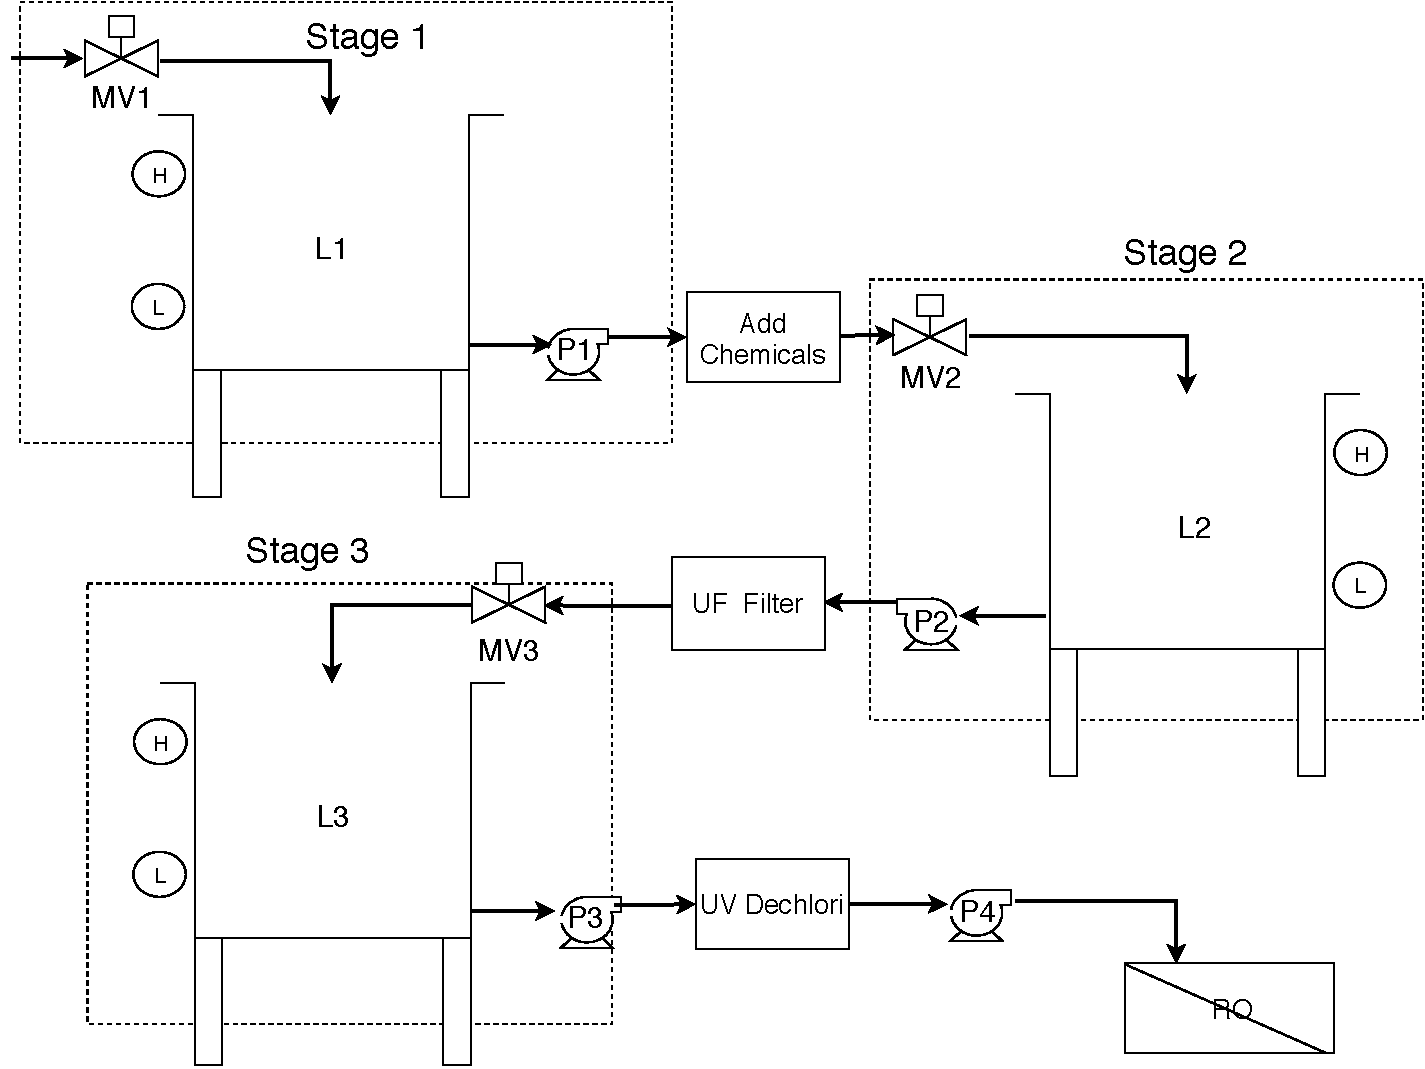
\includegraphics[width=\linewidth]{Figures/SWaT_allTanks-Stages}
  \end{subfigure}
  %
  \begin{subfigure}[b]{.35\linewidth}
  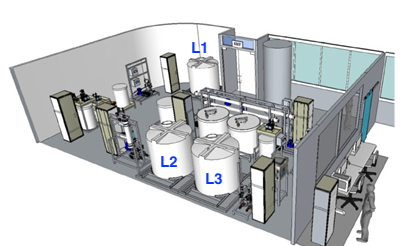
\includegraphics[width=\linewidth]{Figures/testbed.png}
  \end{subfigure}
  %
  \begin{subfigure}[b]{.35\linewidth}
  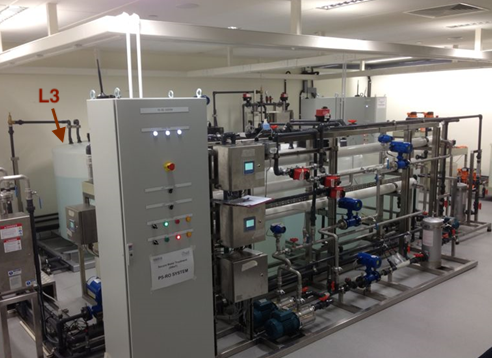
\includegraphics[width=\linewidth]{Figures/testbed2.png}
  \end{subfigure}
  
    \caption{SWaT diagram}
  \label{fig:SWaTSchema}
\end{figure}

%==================END JOHN WORKSPACE====================
%==================BEGIN ERIC WORKSPACE====================
\subsection{SWaT Stage 3}
Recall the motivational example presented in Section~\ref{sec:example} that models Stage 3 of SWaT. We reuse the dynamics presented in Section~\ref{sec:example}, but since there are also pumps and valves in the other process we model (Stage 2), we rename the components, i.e., $MV$, $L$, and $P$ are now respectively $MV3$, $L3$ and $P3$, matching the descriptions in Figure~\ref{fig:SWaTSchema}.

Stage 3 receives water from Stage 2, and the controller of Stage 3 reports to the controller of Stage 2 the following information: the level of water in the tank $T3$ and the state of the valve $MV3$. To model the composition of Stage 3 with Stage 2, we define the behaviour of the communication channels $\vec{a}$, and $\vec{w}$ for Stage 2, and $\vec{b}$ and $\vec{v}$ for Stage 3. Let  
\begin{align}
  \vec{b}[L3](k+1)&\triangleq \vec{q}[L3](k)\\
  \vec{b}[MV3](k+1)&\triangleq \vec{q}[MV3](k)\\
  \vec{w}[L2](k)&\triangleq \vec{v}[L2](k),\\
  Inflow(k)&=\begin{cases}
    0 & \quad \text{if $\vec{w}[L2](k)=0$}\\
    0.31,&\quad \text{if $\vec{x}[MV](k)=\texttt{open}$}\\
    0,&\quad \text{if $\vec{x}[MV](k)=\texttt{closed}$}\\
    0.26,&\quad \text{otherwise}\\
  \end{cases}
\end{align}
where $\vec{v}[L2](k)$ is part of the behaviour description of Stage 2. The inflow of water for $T3$ now depends on the physical state of $T2$; if there is no water in $T2$, there is no inflow.

\todo[inline]{We do not yet define an attacker model for Stage 3, as we will define one for the composition.}
We now formally model Stage 2 and describe its composition with Stage 3. We then characterise an attacker model to measure the robustness of the composition, which we then proceed to redesign and prove that its robustness improves with respect to given the attacker model.

\subsection{A Formal Model of Stage 2}
We provide a model of SWaT Stage 2. This model has three physical components $MV2$, $L2$ and $P2$, and uses the constants $L2min=800$, $L2max=1000$ and $T2=7$.

\paragraph{The Controller $\plc_2$} 
This controller has eight modes which depend on the state of the pump $P2$ and the valve $MV2$, and a timer, so $\vec{q}$ has three coordinates: $P2$, $MV2$, and $\tau2$. Their respective ranges are $\vec{q}[P2]\in\set{\texttt{off},\texttt{on}}$, $\vec{q}[MV2]\in\set{\texttt{closed},\texttt{opening},\texttt{open},\texttt{closing}}$ and $\vec{q}[\tau2]\in\mathbb{N}$. 

The controller $\plc_2$ receives a network input $\vec{a}$ and a sensor reading $\vec{y}$, and produces a control signal $\vec{u}$. Through this section, we assume that every actuator and sensor behaves like a faithful single state transducer, i.e. $\vec{i}(k)=\theta_{\vec{Y}}(\vec{y}(k))=\vec{y}(k)$ and $\vec{u}(k)=\theta_{\vec{O}}(\vec{o}(k))=\vec{o}(k)$.

The network input $\vec{a}$ has two coordinates $L3$ and $MV3$, whose ranges are $\vec{a}[L3]\in[0..1200]$ and $\vec{a}[MV]\in \{\texttt{closed},\texttt{opening},\texttt{open},\texttt{closing}\}$. 

The sensor reading $\vec{y}$ has one coordinate $L2$, where $\vec{y}[L2]\in[0..1200]$. 

The control signal $\vec{u}$ has two coordinates, $MV2$ and $L2$, where $\vec{u}[P2]\in\set{\const_\texttt{off},\const_\texttt{on},\id}$, and $\vec{u}[MV2]\in\set{\texttt{closed},\texttt{opening},\const_\texttt{open},\const_\texttt{closing}, \id}$.
%$\vec{u}[MV2]\in\set{\const_\texttt{closed},\const_\texttt{opening},\const_\texttt{open},\const_\texttt{closing}}$.

We define the behaviour of the controller as follows: let $L3_k=\vec{a}[L3](k)$, $MV3_k=\vec{a}[MV3](k)$, $MV2_k=\vec{q}[MV2](k)$, $P2_k=\vec{q}[P2](k)$, and $L2_k=\vec{y}[L2](k)$.
%The controller has the function $\delta_{\vec{Q}}$, defined by
\begin{align}
  % \delta_{\vec{Q}}&((P2,MV2,\tau_2),(L,MV),L2)\triangleq (P2', MV2',\tau_2'),\text{where}\\
\vec{q}[P2](k+1)&\triangleq
    \begin{cases}
      \texttt{off},&\quad \text{if $L3_k\leq L3min$ or $MV3_k\in \set{\texttt{closed},\texttt{closing}}$},\\
      \texttt{on},&\quad \text{if $L3_k \geq L3min$ or $MV3_k\in \set{\texttt{open},\texttt{opening}}$}\\
      P2_k&\quad \text{otherwise;}
    \end{cases}\\
\vec{q}[MV2](k+1)&\triangleq
  \begin{cases}
    \texttt{opening},&\quad \text{if $MV2_k=\texttt{closed}$ and $L2_k\leq L2min$,}\\
    \texttt{open},&\quad \text{if $MV2_k=\texttt{opening}$ and $\tau2_k>T_2$,}\\
    \texttt{closing},&\quad \text{if $MV2_k=\texttt{open}$ and $L2_k\geq L2max$,}\\
    \texttt{closed},&\quad \text{if $MV2_k=\texttt{closing}$ and $\tau2_k>T_2$,}\\
    MV2&\quad \text{otherwise;}    
  \end{cases}\\
\vec{q}[\tau2](k+1)&\triangleq
\begin{cases}
  \tau2_k+1 &\quad \text{if $MV2_k\in \set{\texttt{opening},\texttt{closing}}$}\\
  0&\quad \text{otherwise;}    
\end{cases}\\
\vec{u}[MV2](k+1)=&\const_{MV2_k},\\%\vec{q}[MV2](k)\\%
\vec{u}[P2](k+1)=&\const_{P2_k}.%\vec{q}[P2](k)\\%
\end{align}
% \begin{align*}
%   \theta_{\vec{Q}}(P2,MV2,t)&\triangleq (\vec{o}[MV2],\vec{o}[P2]), \text{where}\\
%   \vec{o}[MV2]&\triangleq MV2
%     % \begin{cases}
%     %   \texttt{open},&\quad  \text{if $MV2=\texttt{opening}$}\\
%     %   \texttt{close},&\quad\text{if $MV2=\texttt{closing}$}\\  
%     %   \perp,&\quad\text{otherwise;}   
%     % \end{cases},
%   ,\quad \text{and }\quad
%   \vec{o}[P2]\triangleq P2
%   % \begin{cases}
%   %   \texttt{on}(),&\quad  \text{if $P2=\texttt{on}$}\\
%   %   \texttt{off}(),&\quad\text{if $P2=\texttt{off}$}\\  
%   %   \perp,&\quad\text{otherwise;}   
%   % \end{cases}
%   \\ 
%   \beta_{\vec{Q}}(P2,MV2,t) &\triangleq \perp.
% \end{align*}
% \paragraph{The Actuators} We have two actuators, the pump $P2$ and the motor valve $MV2$. Their  behaviour is modelled by the function $\theta_{\vec{O}}$, defined for $\vec{o}=(MV2,P2)$ by
% \begin{align}
%   \theta_{\vec{O}}(MV2,P2)&\triangleq (\vec{u}[MV2],\vec{u}[P2]), \text{where}\\
%   \vec{u}[MV2]&\triangleq 
%     \begin{cases}
%       \const_{MV2},&\quad  \text{if $MV2\neq\perp$,}\\
%       \id,&\quad\text{otherwise;}   
%     \end{cases},\\
%   \vec{o}[P2]&\triangleq 
%   \begin{cases}
%     \const_{P2},&\quad  \text{if $P2\neq \perp$,}\\
%     \id,&\quad\text{otherwise;}   
%   \end{cases},
% \end{align}

\paragraph{The Process} 
The state of the process $\vec{x}$ has three coordinates: $L2, MV2$ and $P2$. Their respective ranges are $\vec{x}[L2]\in [0..1200]$, $\vec{x}[MV2]\in \{\texttt{closed},\texttt{opening},\texttt{open},\texttt{closing}\}$ and $\vec{x}[P2]\in \set{\texttt{on},\texttt{off}}$. 
% subcomponents $\vec{x}=(L2,MV2,P2)$, with $\range(\vec{x}[L2])=[0..1200]$, $\range(\vec{x}[MV2])=\set{\texttt{closed},\texttt{opening},\texttt{open},\texttt{closing}}$, and $\range(\vec{x}[P2])=\set{\texttt{on},\texttt{off}}$. 

We leave the initial condition abstract for now. The behaviour of the process is given by
\todo[inline]{@Eric:The initial state of the process is $\vec{x_0}=(990,\texttt{open},\texttt{on})$.}
%The process reacts to the control input $\vec{u}$,

% The process has the function $\delta_{\vec{X}}$, which computes the of value of $\vec{x}(k+1)$ from $\vec{x}(k)$, $\vec{u}[MV2](k)$ and $\vec{u}[P2](k)$
Let $P2_k=\vec{x}[P2](k)$, $MV2_k=\vec{x}[MV2](k)$, and $L2_k=\vec{x}[L2](k)$, and let $\delta_{P2}=\vec{u}[P2](k)$, and $\delta_{MV2}=\vec{u}[MV2](k)$; we define the behaviour of the process by
\begin{align*}
  %\delta_{\vec{X}}&((L2,MV2,P2),(\vec{u}[MV2],\vec{u}[P2]))\triangleq (L2', MV2',P2'),\text{where}\\
\vec{x}[P2](k+1)&\triangleq \delta_{P2}(P2_k)\\
\vec{x}[MV2](k+1)&\triangleq \delta_{MV2}(MV2_k)\\
\vec{x}[L2](k+1)&\triangleq L2_k+\partial(MV2_k,P2_k),\text{where}\\
\partial(MV2,P2)&\triangleq
\begin{cases}
  0&\quad \text{if $MV2_k=\texttt{closed}$ and $P2_k=\texttt{off}$}\\
  0.46&\quad \text{if $MV2_k=\texttt{open}$ and $P2_k=\texttt{off}$}\\
  0.29&\quad \text{if $MV2_k\in\set{\texttt{opening},\texttt{closing}}$ and $P2_k=\texttt{off}$}\\
  -0.29&\quad \text{if $MV2_k=\texttt{closed}$ and $P2_k=\texttt{on}$}\\
  0.13&\quad \text{if $MV2_k=\texttt{open}$ and $P2_k=\texttt{on}$}\\
  -0.28&\quad \text{if $MV2_k\in\set{\texttt{opening},\texttt{closing}}$ and $P2_k=\texttt{on}$}\\  
\end{cases}
\end{align*}
The values for $\partial(MV2,P2)$ were computed by linear regression in \cite{John?}
\footnote{ \todo[inline]{@John: can you plese provide the right reference?}} 
to approximate the flow equation $L2_{k+1}=L2_{k}+\texttt{Inflow}_k-\texttt{Outflow}_k$.

The sensor reading $\vec{y}$ has only one coordinate $L2$, whose range is $\vec{y}\in \mathbb{R}^+$; i.e, any positive value. The behaviour of $\vec{y}$ is given by 
\begin{align}
  \vec{y}[L2](k)=\vec{x}[L2]
\end{align}

Finally, the physical state of the process propagates to Stage 3 via the abstract channel $\vec{v}[L3]$
\begin{align}
  \vec{v}[L2](k)&\triangleq \vec{x}[L2](k)
\end{align}
\todo[inline]{@All. Reviewers might ask why we do not include errors in the models. They can be added, but I wanted to keep the model as simple as possible.}

% The process produces the output $\theta_{\vec{X}}$, defined by
% \begin{align*}
%   \theta_{\vec{X}}(\vec{x})\triangleq \vec{y}[L2], \text{where $\vec{y}[L2]=\vec{x}[L2]$}.
% \end{align*} 
% \paragraph{Sensors} Finally, the behaviour of the water level sensor is given by the function $\theta_{\vec{Y}}$, defined by 
% \begin{align*}
%   \theta_{\vec{Y}}(\vec{y})\triangleq \vec{i}[L2]\text{, where $\vec{i}[L2]=\vec{y}[L2]$.}
% \end{align*}

\begin{figure}[t]
  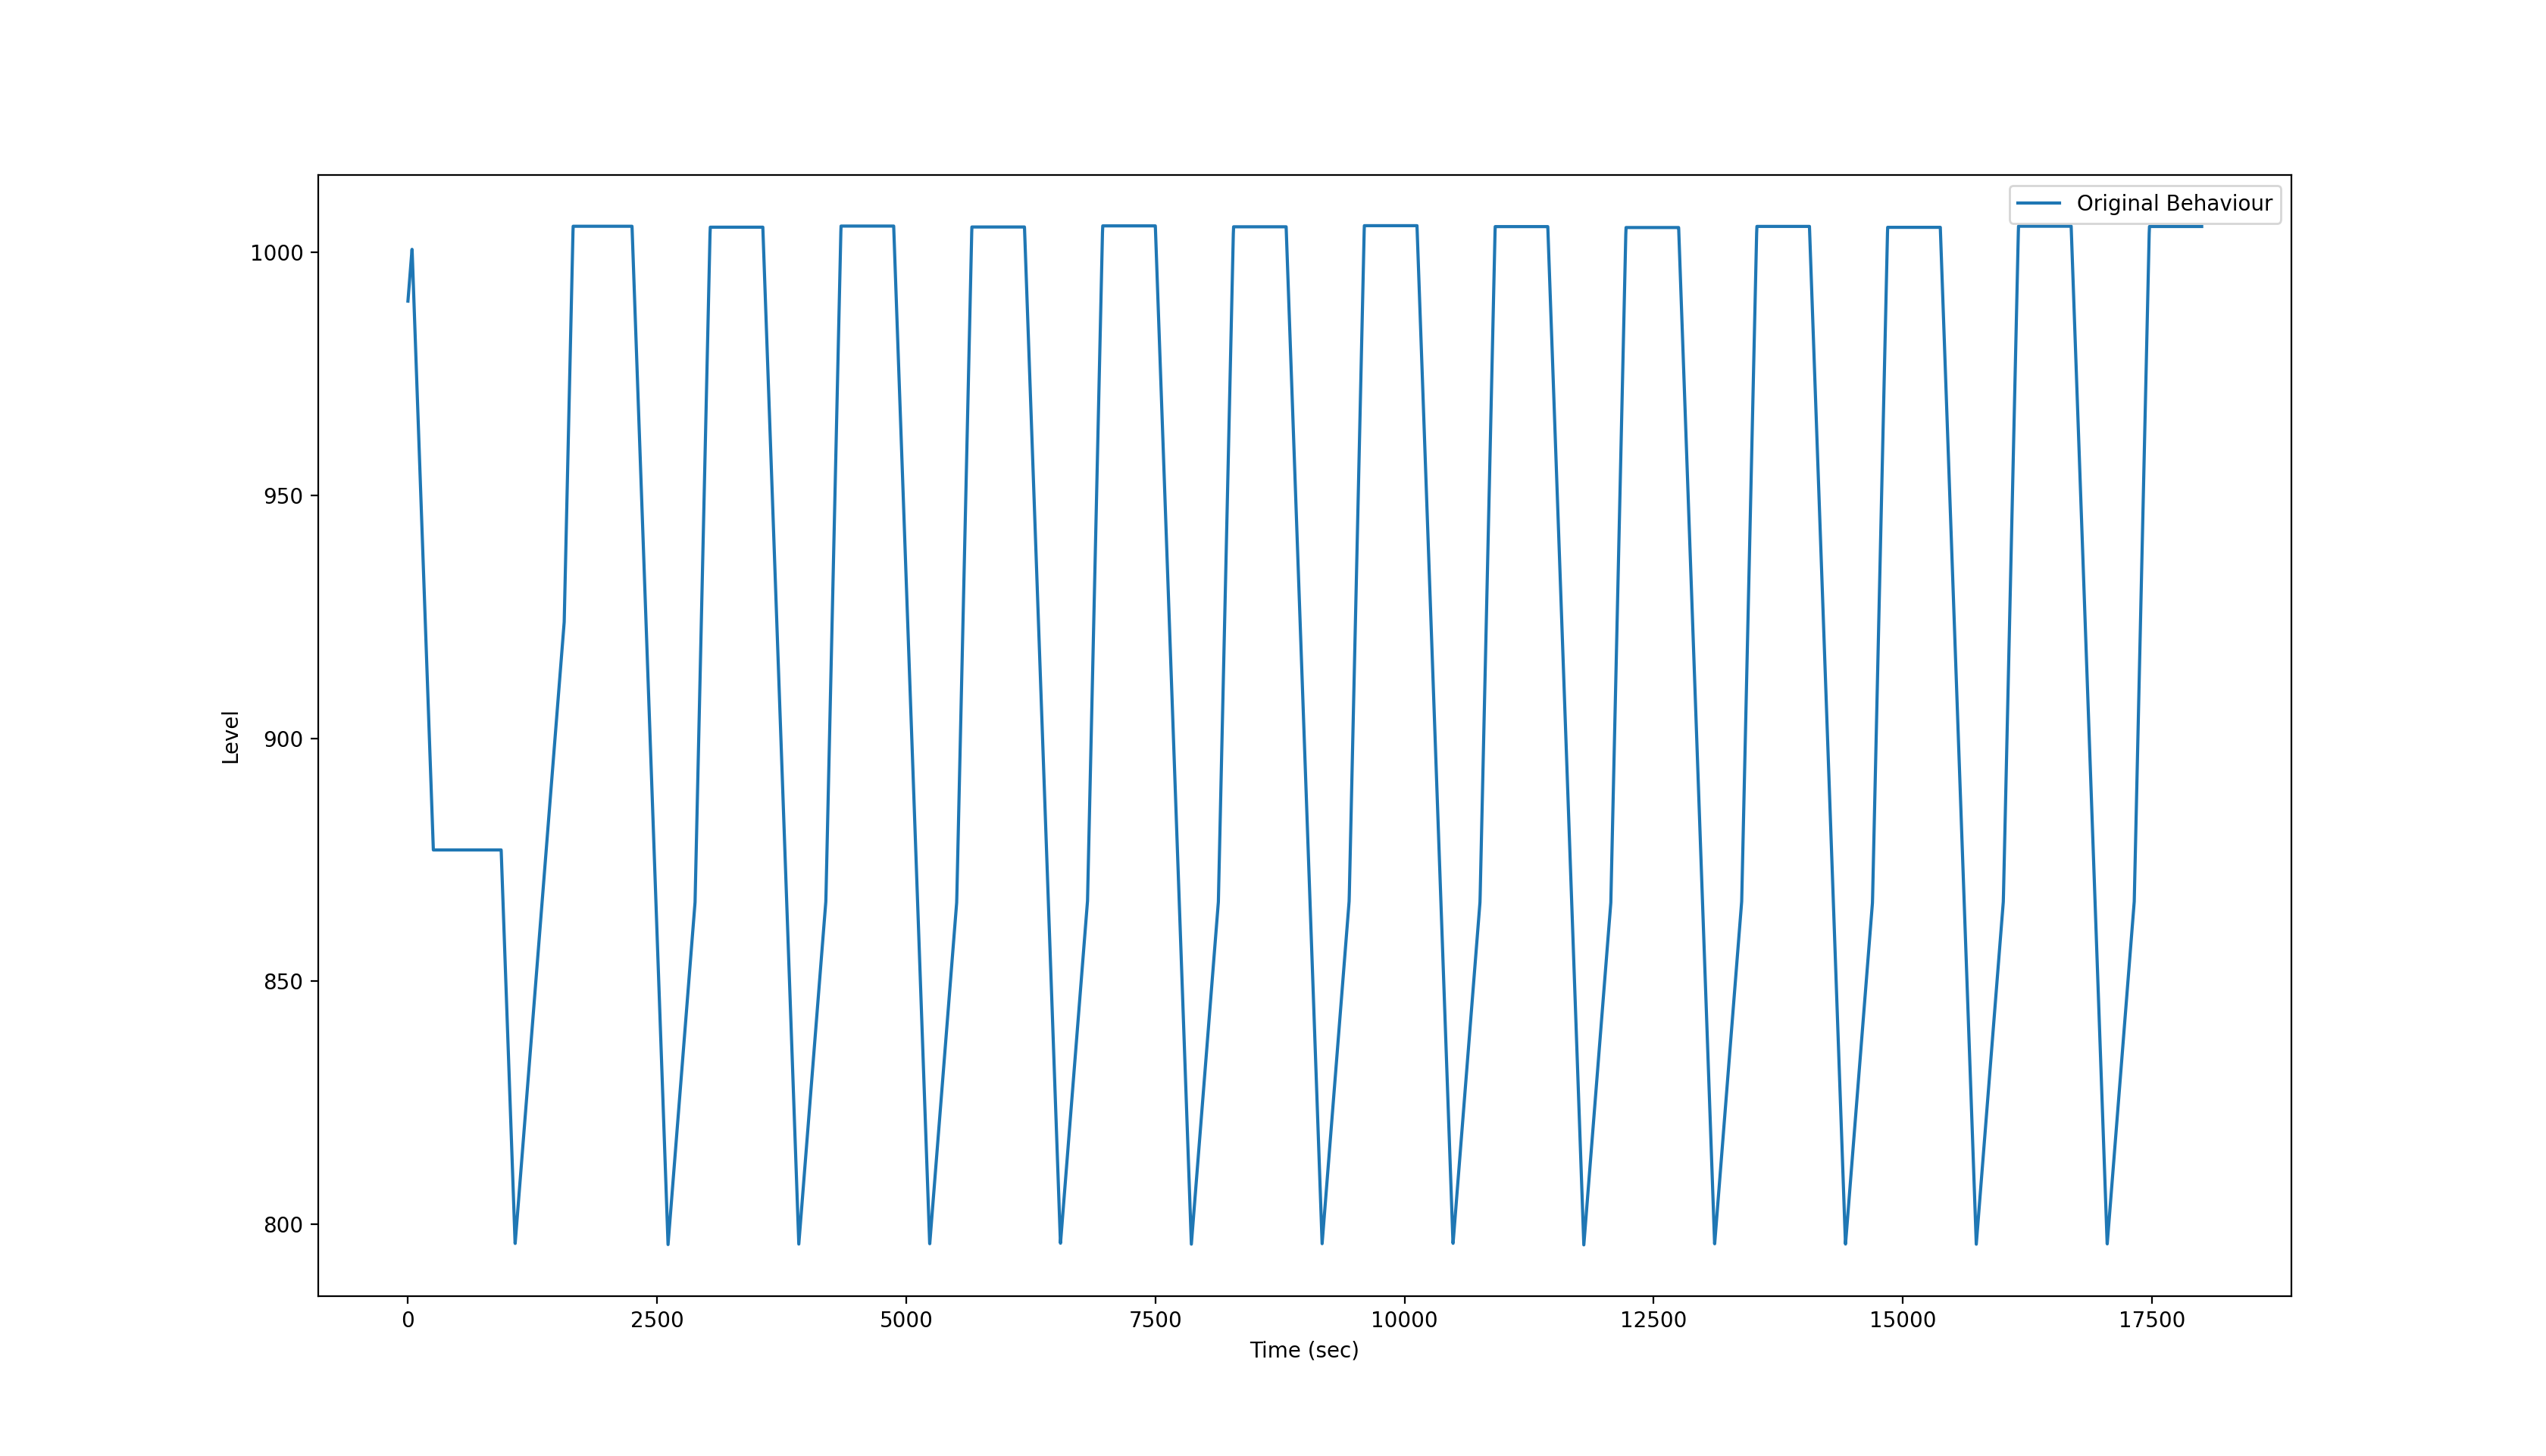
\includegraphics[width=0.75\textwidth]{Figures/Stage2Normal.png}
  \caption{Normal behaviour of the water level of Stage 2 if Stage 3 is also operating normally.}
  \label{fig:Stage2Normal}
\end{figure}
Under normal circumstances, the water level of tank T2 exhibits the behaviour shown in Figure~\ref{fig:Stage2Normal}.

% The controller has the output functions $\beta_{\vec{Q}}$ and $\theta_{\vec{Q}}$, defined by
% \begin{align}
%   \theta_{\vec{Q}}(P2,MV2,t)&\triangleq (\vec{o}[MV2],\vec{o}[P2]), \text{where}\\
%   \vec{o}[MV2]&\triangleq 
%     \begin{cases}
%       \texttt{open}(),&\quad  \text{if $MV2=\texttt{opening}$}\\
%       \texttt{close}(),&\quad\text{if $MV2=\texttt{closing}$}\\  
%       \perp,&\quad\text{otherwise;}   
%     \end{cases},\\
%   \vec{o}[P2]&\triangleq P2\\ 
%   \beta_{\vec{Q}}(P2,MV2,t) &\triangleq \perp.
% \end{align}

\subsection{Attacker Model}%{Some Attacker Models of Stage 2 and Stage 3}
% We define an attacker model for the composition of Stage 2 and Stage 3 by combining two attacker models, one for Stage 2 and one for Stage 3.  The following models describe single-point attackers in one of the processes.
We now define an attacker model using Definitions~~\ref{def:AttackBasis},\ref{def:IdempotentMonoid}, and~\ref{def:Attack} for the quantification of robustness. We have four security requirements: $\Always{\vec{x}[L2]>0}$, $\Always{\vec{x}[L2]<1200}$, $\Always{\vec{x}[L3]>0}$ and $\Always{\vec{x}[L3]<1200}$. We consider an attacker model that can manipulate the control outputs of the controller PLC2 for pump $P2$ and valve $MV2$; i.e. the attacker can set $\vec{u}[MV2](k)$ and $\vec{u}[P2](k)$ for all $0\leq k\leq t$ given some testing time parameter $t$, which we set to 6 hours to give the effect of actions of the attacker enough time to propagate through the system. We reuse the base from Example~\ref{ex:AttackBasis}: the base for the attacker model is $[LL, OK, HH]^T$, where ${LL}(\pi)=\pi[\vec{x}[L3]]<L3min$, ${HH}(\pi)=\pi[\vec{x}[L3]]>L3max$ and ${OK}(\pi)=L3min \leq \pi[\vec{x}[L3]]\leq L3max$, for $\pi \in \Pi$. This implies that even though the attacker modifies components in Stage2, they only have visibility of the tank T3 and not of T2. Although this attacker is ``blind" with respect to $T2$, their actions will definitely impact the behaviour of $T2$. 

We define the representative values of $\vec{u}[MV2]$ to be $\texttt{open}$, and $\texttt{closed}$; more precisely, we define
\begin{align*}
  \Gamma_{\vec{u}[MV2]}=\set{\const^{\vec{u}[MV2]}_{\texttt{open}}, \const^{\vec{u}[MV2]}_{\texttt{closed}}}.
\end{align*}
We also define the representative values of $\vec{u}[P2]$ to be $\texttt{on}$, and $\texttt{off}$, yielding the constant functions; i.e., 
\begin{align*}
  \Gamma_{\vec{u}[P2]}=\set{\const^{\vec{u}[P2]}_{\texttt{on}}, \const^{\vec{u}[P2]}_{\texttt{off}}}.
\end{align*}
% The set of coefficients for this attacker model is $\Gamma_{\vec{u}[MV2],\vec{u}[P2]}=\Gamma_{\vec{u}[MV2]}\cup \Gamma_{\vec{u}[P2]}$. 
The attacks of this attacker model $\vec{m}$ are then of the form
\begin{align*}
  \vec{m}(\pi)=
  %[t_1,\ldots,t_n]
  \begin{bmatrix}
    t_1\circ s_1 \\
    t_2\circ s_2 \\
    t_3\circ s_3 \\
  \end{bmatrix}
  \cdot
  \begin{bmatrix}
    LL \\
    OK \\
    HH
  \end{bmatrix},
\end{align*} 
where $t_i\in \set{\id,\const^{\vec{u}[MV2]}_{\texttt{open}}, \const^{\vec{u}[MV2]}_{\texttt{closed}}}$ and  $s_i\in\set{\id,\const^{\vec{u}[P2]}_{\texttt{on}}, \const^{\vec{u}[P2]}_{\texttt{off}}}$, for $i\in \set{1,2,3}$. The resulting attacker model has 729 attacks because
 \begin{align*}
  \left| \IM{\Gamma_{\set{\vec{u}[MV2],\vec{u}[P2]}}}\right|^{\left|\set{{LL},{OK},{HH}}\right|}=9^3=729.
\end{align*}

\subsection{Counter Attacker Model}
The corresponding counter attacker model uses the controller PLC3; i.e. the counter attacker can set $\vec{q}[MV3](k)$ and $\vec{q}[P3](k)$ for all $0\leq k\leq t$ , with  $t=6$ hours to let the actions of the attacker and counter attacker enough time to stabilise. Since the counter attacker is in the controller of Stage 3, we define the base for the counter attacker model to be $[LL', OK', HH']^T$, where ${LL'}(\pi)=\pi[\vec{y}[L3]]<L3min$, ${HH'}(\pi)=\pi[\vec{y}[L3]]>L3max$ and ${OK'}(\pi)=L3min \leq \pi[\vec{y}[L3]]\leq L3max$, for $\pi \in \Pi$ (unlike the base of the attacker, which uses $\vec{x}[L3]$ instead of $\vec{y}[L3]$). The counter attacker is also ``blind" with respect to $T2$, but their actions also impact the behaviour of $T2$. 

We set the representative values of $\vec{q}[MV3]$ to be $\texttt{open}$, and $\texttt{closed}$ and the representative values of $\vec{q}[P3]$ to be $\texttt{on}$, and $\texttt{off}$; more precisely, 
\begin{align*}
  \Gamma_{\vec{q}[MV3]}&=\set{\const^{\vec{u}[MV3]}_{\texttt{open}}, \const^{\vec{u}[MV3]}_{\texttt{closed}}}.\\
  \Gamma_{\vec{q}[P3]}&=\set{\const^{\vec{u}[P3]}_{\texttt{on}}, \const^{\vec{u}[P3]}_{\texttt{off}}}.
\end{align*}
% The set of coefficients for this attacker model is $\Gamma_{\vec{u}[MV2],\vec{u}[P2]}=\Gamma_{\vec{u}[MV2]}\cup \Gamma_{\vec{u}[P2]}$. 
The counter attacks of this model $\vec{w}$ are then of the form
\begin{align*}
  \vec{w}(\pi)=
  %[t_1,\ldots,t_n]
  \begin{bmatrix}
    t_1\circ s_1 \\
    t_2\circ s_2 \\
    t_3\circ s_3 \\
  \end{bmatrix}
  \cdot
  \begin{bmatrix}
    LL' \\
    OK' \\
    HH'
  \end{bmatrix},
\end{align*} 
where $t_i\in \set{\id,\const^{\vec{q}[MV3]}_{\texttt{open}}, \const^{\vec{q}[MV3]}_{\texttt{closed}}}$ and  $s_i\in\set{\id,\const^{\vec{u}[P3]}_{\texttt{on}}, \const^{\vec{u}[P3]}_{\texttt{off}}}$, for $i\in \set{1,2,3}$. This counter attacker model has 729 counter attacks.

\subsection{Quantification of Robustness: Analysis of Results}
Using LBA, we quantify the robustness of the system given the initial conditions $\vec{x}[L2]=990$, $\vec{x}[MV2]=open$, $\vec{x}[P2]=on$, $\vec{x}[L3]=920$, $\vec{x}[MV3]=open$, $\vec{x}[P3]=on$. The robustness factor of 162/729, meaning that are successful 567 attacks for the given attacker model. All attacks that break $\Always{\vec{x}[L3]>0}$ or $\Always{\vec{x}[L3]<1200}$ can always be countered. However, 148 attacks cannot be countered by the proposed attacker model, meaning that the latent robustness of the system is $581/729$. Non countered attacks always break either $\Always{\vec{x}[L2]>0}$ or $\Always{\vec{x}[L2]<1200}$. Nevertheless, some attacks which break $\Always{\vec{x}[L2]>0}$ or $\Always{\vec{x}[L2]<1200}$ can be countered. For example, the following attack $\vec{m}$ breaks the requirement $\Always{\vec{x}[L2]<1200}$, but it is countered by the following counter attack $\vec{w}$ 
\begin{align*}
%   Requirement "Tank T2 Never Overflows" broken at time 644 by attack (x[L3]<L3min)=>[(O[P2]->off), (O[MV2]->open)] + (L3min<=x[L3]<=L3max)=>[id(O[P2]), id(O[MV2])] + (x[L3]>L3max)=>[id(O[P2]), id(O[MV2])]
% Found counterattack(Y[L3]>L3max)=>[id(Q[MV3]), (Q[P3]->off)] + (L3min<=Y[L3]<=L3max)=>[id(Q[MV3]), id(Q[P3])] + (Y[L3]<L3min)=>[id(Q[MV3]), id(Q[P3])]
  \vec{m}(\pi)&=
  %[t_1,\ldots,t_n]
  \begin{bmatrix}
   \const^{\vec{u}[MV2]}_{\texttt{open}}\circ \const^{\vec{u}[P2]}_{\texttt{off}} \\
   \id\circ \id \\
   \id\circ \id \\
  \end{bmatrix}
  \cdot
  \begin{bmatrix}
    \pi[\vec{x}[L3]]<L3min \\
    L3min \leq \pi[\vec{x}[L3]]\leq L3max \\
    \pi[\vec{x}[L3]]>L3max
  \end{bmatrix},\\
  \vec{w}(\pi)&=
  %[t_1,\ldots,t_n]
  \begin{bmatrix}
    \id\circ \id \\
    \id\circ \id \\
    \id\circ \const^{\vec{q}[P3]}_{\texttt{off}} \\
  \end{bmatrix}
  \cdot
  \begin{bmatrix}
    \pi[\vec{y}[L3]]<L3min \\
    L3min \leq \pi[\vec{y}[L3]]\leq L3max \\
    \pi[\vec{y}[L3]]>L3max
  \end{bmatrix}.
\end{align*} 
The following attack $\vec{m}'$ cannot be countered using the current counter attacker model,
\begin{align*}
  %(x[L3]<L3min)=>[id(O[P2]), id(O[MV2])] + (L3min<=x[L3]<=L3max)=>[(O[P2]->off), (O[MV2]->open)] + (x[L3]>L3max)=>[(O[P2]->off), id(O[MV2])]
    \vec{m}'(\pi)&=
    %[t_1,\ldots,t_n]
    \begin{bmatrix}
     \id\circ \id \\
     \const^{\vec{u}[MV2]}_{\texttt{open}}\circ \const^{\vec{u}[P2]}_{\texttt{off}} \\
     \id\circ \const^{\vec{u}[P2]}_{\texttt{off}} \\
    \end{bmatrix}
    \cdot
    \begin{bmatrix}
      \pi[\vec{x}[L3]]<L3min \\
      L3min \leq \pi[\vec{x}[L3]]\leq L3max \\
      \pi[\vec{x}[L3]]>L3max
    \end{bmatrix}.
  \end{align*} 
\todo[inline]{provide concrete examples of attacks.}

\subsection{Increasing Robustness}
LBA reveals that several attacks that empty tank T3 can be countered by means of the counter attack 
\begin{align*}
  %(Y[L3]>L3max)=>[id(Q[MV3]), (Q[P3]->off)] + (L3min<=Y[L3]<=L3max)=>[id(Q[MV3]), id(Q[P3])] + (Y[L3]<L3min)=>[id(Q[MV3]), id(Q[P3])]
    \vec{w}'(\pi)&=
    %[t_1,\ldots,t_n]
    \begin{bmatrix}
    \id\circ \const^{\vec{q}[P3]}_{\texttt{off}} \\
     \id\circ \id \\
     \id\circ \id \\
    \end{bmatrix}
    \cdot
    \begin{bmatrix}
      \pi[\vec{x}[L3]]<L3min \\
      L3min \leq \pi[\vec{x}[L3]]\leq L3max \\
      \pi[\vec{x}[L3]]>L3max
    \end{bmatrix},
  \end{align*} 
which is sensible: if the tank $T3$ is losing water, by shutting off the pump $P3$ when the level is low, we prevent water from leaving the tank.

Several attacks countered by this counter attack share the factor $(\const^{\vec{u}[P2]}_{\texttt{off}})(\vec{x}[L3]]<L3min)$, which is why we propose to apply the counter attack $\vec{w}'$ only when $\vec{u}[P2]$ is \texttt{off} and $\vec{x}[L3]]<L3min$. To implement this counter attack, we empower the controller PLC3 to set $\vec{q}[P3]$ to \texttt{off} if $\vec{u}[P2]$ is \texttt{off} and $\vec{y}[L3]]<L3min$; we use $\vec{y}[L3]]<L3min$ instead of $\vec{x}[L3]]<L3min$ because $\vec{y}[L3]=\vec{x}[L3]$, PLC3 has access to $\vec{y}[L3]$, and because the attacker model does not include $\vec{y}[L3]$. These changes increase the robustness of the system from 162/729 to 270/729, since the controller PLC3 now prevents the tank T3 from running out of water due to the effect of 108 attacks that broke this requirement in the original system. The latent robustness remains at 581/729, which means that implementing this counter attack did not add additional vulnerabilities.


% (Y[L3]>L3max)=>[id(Q[MV3]), (Q[P3]->off)] + (L3min<=Y[L3]<=L3max)=>[id(Q[MV3]), id(Q[P3])] + (Y[L3]<L3min)=>[id(Q[MV3]), id(Q[P3])]
% because
%  \begin{align*}
%   \left| \IM{\Gamma_{\set{\vec{u}[MV2],\vec{u}[P2]}}}\right|^{\left|\set{{LL},{OK},{HH}}\right|}=9^3=729.
% \end{align*}

% \begin{align*}
%   \vec{m}=&(x[L3]<L3min)(\gamma_1(\vec{u}[P2]), \gamma_1(\vec{u}[P2]) + \\
%   &(L3min\leq x[L3]leq L3max)(\gamma_2(\vec{u}[P2]), \gamma_2(\vec{u}[P2]) + \\
%   &(x[L3]>L3max)(\gamma_3(\vec{u}[P2]), \gamma_3(\vec{u}[P2])
% \end{align*}
% % We are mostly interested in discovering attackers that can affect the physical state $\vec{x}$ without physical interaction. We cannot effectively defend from the cyber part of the CPS (e.g. by redesigning the controller, or by adding more sensors) against attackers that can directly manipulate the physical state, because their attackers can bypass the controller. Therefore, we assume that we can protect the physical components of a CPS though physical security, and we assume that attackers are not able to directly corrupt physical component%(i.e. $\vec{u}, \vec{x}, \vec{y}, \vec{v}$ and $\vec{w}$)
% % , so their attacks must be carried out by corrupting non-physical components.% (i.e. $\vec{a}, \vec{b},\vec{i}, \vec{q}$ and $\vec{o}$).

% More precisely,  
% %if the state of a CPS has vectors $\vec{a},\vec{b},\vec{i},\vec{o}, \vec{u}, \vec{y}, \vec{v},\vec{w},\vec{q}$, and $\vec{x}$,
% we define attackers for this CPS over the following set of components 
% \begin{align}
%   \Sigma_{0}=\set{\vec{i}[L2], \vec{a}[L], \vec{a}[MV], \vec{q}[P2], \vec{q}[MV2], \vec{q}[\tau_2], \vec{o}[MV2], \vec{o}[P2]}.
% \end{align}
% We define the partition of states $\set{(L2< L2min),(L2min\leq L2\leq L2max),(L2>L2max)}$ to allow the definition of attacks based on these three predicates over states as explained in Definition~\ref{def:Attack}. 

% We chose arbitrary ranges for the vulnerable components in $\Sigma_0$ so that they can have different effects on the controller. For example, $\widehat{\vec{i}[L2]}\triangleq\set{700,900,1100}$, since we evaluate whether $L2 \leq L2min$ and $L2 \geq L2max$, and $L2min=800$ and $L2max=1000$. The ranges for all the vulnerable components are the following:
% \begin{align*}
%   \widehat{\vec{i}[L2]}&\triangleq\set{700,900,1100}\\
%   \widehat{\vec{a}[L]}&\triangleq\set{700,900,1100}\\
%   \widehat{\vec{a}[MV]}&\triangleq\range(\vec{a}[MV])\\
%   \widehat{\vec{q}[P2]}&\triangleq\range(\vec{q}[P2])\\
%   \widehat{\vec{q}[MV2]}&\triangleq\range(\vec{q}[MV2])\\
%   \widehat{\vec{q}[\tau_2]}&\triangleq\set{0,7}\\
%   \widehat{\vec{o}[MV2]}&\triangleq\range(\vec{o}[MV2])\\
%   \widehat{\vec{o}[P2]}&\triangleq\range(\vec{o}[P2]).
%   %\set{ \vec{a}[L], \vec{a}[MV], \vec{q}[P2], \vec{q}[MV2], \vec{q}[\tau_2], \vec{o}[MV2], \vec{o}[P2]}.
% \end{align*}
% Let us first consider attacks that affect only one component. 
% Under this configuration, we generate 1161 attacks on individual components. We present the manifested latent behaviours of these attacks that can break either of the requirements $\Always{\vec{x}[L2]>0}$ or $\Always{\vec{x}[L2]<1200}$ in Figure~\ref{fig:DangerousLatentBehavioursStage2}.
% \begin{figure}[t]
%   \includegraphics[width=\textwidth]{Figures/LevelT2-Stage2Attackers-OnlySuccessfulAttacks-OverUnderflowL2-3Partition.png}
%   \caption{Latent behaviours manifested by attacks on the components of Stage 2. All these latent behaviours break either the overflow or the empty tank requirement.}
%   \label{fig:DangerousLatentBehavioursStage2}
%   \end{figure}

% \todo[inline]{
%   Successful attackers with only one component= ${'PLC2[timer]', 'PLC2[mode]', 'O[MV2]', 'L2[level]'}$Analysis finished in 399.3336 seconds.
%   There are 393 successful attacks under state partition ${'L2>L2max', 'L2<L2min', 'L2min<=L2<=L2max'}$
% Tested 1161 attacks in total
% }

% Both Stage 2 and Stage 3 have invariant security requirements: their respective tanks must never be empty and the tanks must never overflow. 

% \subsubsection{Attacking Stage 2}.

% \subsubsection{Attacking Stage 2 from Stage 3}. The results are interesting. There are NO invariant attacks from stage 3 to stage 2, but there are a couple of conditional attacks! The following attacks work because the state of MV sent to Stage 2 depends on the mode of PLC3, and that is what the attacker changes. 
% \begin{itemize}
%   \item stop condition T2\_overflow triggered at time 20658 for attack P.Q[mode]=(L2<L2min)=>id, (L2>L2max)=>(=open), (L2min<=L2<=L2max)=>(=open), 
%   \item stop condition T2\_overflow triggered at time 20657 for attack P.Q[mode]=(L2<L2min)=>id, (L2>L2max)=>(=opening), (L2min<=L2<=L2max)=>(=open), 
%   \item stop condition T2\_overflow triggered at time 20658 for attack P.Q[mode]=(L2<L2min)=>(=closing), (L2>L2max)=>(=open), (L2min<=L2<=L2max)=>(=open), 
%   \item stop condition T2\_overflow triggered at time 20657 for attack P.Q[mode]=(L2<L2min)=>(=closing), (L2>L2max)=>(=opening), (L2min<=L2<=L2max)=>(=open), 
%   \item stop condition T2\_overflow triggered at time 20658 for attack P.Q[mode]=(L2<L2min)=>(=closed), (L2>L2max)=>(=open), (L2min<=L2<=L2max)=>(=open), 
%   \item stop condition T2\_overflow triggered at time 20657 for attack P.Q[mode]=(L2<L2min)=>(=closed), (L2>L2max)=>(=opening), (L2min<=L2<=L2max)=>(=open), 
% \end{itemize}

% \todo[inline]{
%   There are 6 successful attacks under state partition {'L2<L2min', 'L2>L2max', 'L2min<=L2<=L2max'}
% Tested 341 attacks in total
% We tested these attackers= {'PLC3[mode]', 'PLC3[timer]', 'O[MV]', 'L[level]'}
% Successful attackers with only one component= {'PLC3[mode]'}
% Analysis finished in 189.1896 seconds
% }

%==================END ERIC WORKSPACE====================

\section{Discussion and Future Work}
\label{sec:Discussion}
In this section, we list and discuss some fundamental discussion points, some of which represent the basis for interesting future work. 
\todo[inline]{We do not work with attackers that act on physical components.}
\todo[inline]{We do not provide heuristics to choose the most pressing attacker to be addressed.}
\todo[inline]{As we briefly mentioned in Section~\ref{sec:example}, partitioning the state space could be automated by means of data-flow analysis of the controller; more precisely, by determining the path conditions of the program of controller, as illustrated in \cite{John?}. Moreover, the transformations can be systematically obtained by a fuzzying framework (e.g.\cite{AFL}) or by symbolic/concolic execution (e.g. \cite{SymbolicExecutionInCPS?}).}

{\color{red}
\subsection{Modelling and Abstraction level}
Although we provide a formal framework for the modelling of CPSs, their states, and their execution semantics, and showed evidence that it can be used to derive useful analysis, it will be a subject of future work to assess how appropriate our modelling is when applied to other, perhaps more complex, scenarios. In essence, our formalism defines a deterministic transition system whose transition function is given by the one-step cycle semantics function $\TheSystem$ (see Definition \ref{def:SingleCycleSemantics}). Consequently, the notion of integrity that we use in Definition \ref{def:NICPS} is not probabilistic. However, we believe that this approach is good enough to carry out an approximate analysis if the probabilistic nature of the process is due to the existence of zero-mean noises.

\emph{Hybrid automata} \cite{ALUR19953} are state-based models for dynamical systems. These automata allow the description of invariants and side-effects on transitions, making them suitable for the description of many continuous physical processes. There are also model checking techniques for hybrid automata. It would be interesting to see if these automata provide any advantages when it comes to automatic verification of the proposed properties.

\subsection{Quantification of Interference}
For our case study, we came up with a notion of quantification of integrity violations which, ultimately, was related to how many unwanted states could an attacker force the system to be in, in other words the level of \emph{corruption} an attacker can induce. These metrics are in a sense dual to metrics used in quantitative information flow, which measure the entropy of information, and how likely it is for an attacker to guess a secret based on the information she has already observed. 

Ideally, we want to quantify the $k$-controllability of attackers for large values of $k$ in order to cover as many possible states. Unfortunately, the larger $k$ is, the more computationally demanding the analysis becomes. However, we want to highlight that the behaviour of CPSs is usually regular; \emph{i.e.}, the operation modes of CPSs often follow the same sequence over and over, revisiting similar states each time the process repeats. Due to this regular nature, it may be possible to restrict the analysis to the length of this ``behavioural loop'' instead of analysing arbitrarily long traces, therefore considering a well defined and relatively small $\bar{k} \in \mathbb{N}$.

\subsection{A Theory of Attacks and Attackers}
From our case study, we observe that it is possible for different attackers to drive the CPS to critical states by using different attack strategies. Thus, it may be convenient to define more abstract notions of attack and attacker that are more related to the effects that we want to avoid on the system in order to bundle together attacks and attackers that are equally powerful.
While we think that our attacker model is at least as powerful as attacker models commonly used in control theory (see Section \ref{sec:AttacksOnModels}), further work is indeed to formally compare them. 

\subsection{Properties}
There are many well-known properties in control theory that characterise important aspects of dynamical systems, including {controllability, observability, stability} and {stabilizability}. Since we focus on the protection of the integrity of the process, we want to reduce the degree of \emph{controllability} that the attacker has over the system. A focus on the protection of the confidentiality of data would aim to reduce the degree of \emph{observability} that the attacker has over the system. Krotofil and Larsen acknowledge the importance of reasoning about {controllability} and {observability}, but they highlight that it is also important to reason about \emph{operability}, which is ``the ability to achieve acceptable operations'' \cite{krotofil2015rocking}. Determining how our notion of process integrity relates to these other properties is an interesting research topic.

\subsection{Proof Automation}
{From the manual analysis of the case study CPS in the previous section, we foresee that it will be possible to use existing techniques (such as automated theorem proving, model-checking, model counting, and SMT solving) to automate parts of the verification. The definition of the measures for quantification, the notions of critical state, the attackers and the initial states must naturally be done manually, but the problem of verification can be reduced to the quantification of the reachable states by an attacker (similar as in quantitative information flow analysis for confidentiality). We want to first focus on the characterisation of the $k$-controllability of the attacker over the system, since it needs to be computed only once, and then we can apply different security measures to the resulting set of reachable states.}

It would be also interesting to determine whether our approach together with state-of-the-art verification tools has advantages over existing control-theoretical reasoning techniques, which focus on solving algebraic 
representations of CPSs.

\subsection{Redesign}
In our case study, we determined that the attacker $\alpha_3$ was more powerful than the attacker $\alpha_2$ due to the way the controller was designed. Thus, we believe that it would be interesting to develop a methodology for (re)designing controllers that helps avoiding these type of unsafe behaviours. 
}
\section{Related Work}
\todo[inline]{We have to really define what out contribution is W.R.T existing tools that do testing/simulation/symbolic execution/etc. Compare against \url{https://ths.rwth-aachen.de/research/tools/}}
\todo[inline]{@John: Please review this following part in blue.}
\todo[inline]{@ALL: do you know any fuzzying tool/paper besides AFL(Fast) that should always be cited? If you know of any relevant references, please feel free to add them here.}
{\color{blue}
\subsection{Tools for Reachability Analysis of Hybrid Systems}
We do not use hybrid automata. We may be questioned why, since we are working on CPS. However, it is not that we cannot use hybrid automata; we just wanted to separate the cyber part as much as we could from the physical part, because we wanted to easily define interaction points between attackers and system. If those interaction points are clear in hybrid automata, we should do it too for them; e.g., if a sensor is modelled as some state variable of a mode, then an attacker of that sensor should be able to modify that property of the current mode. In other words, attacks are transformations of the state variables of modes. However, it may be more complicated: an attacks might need to satisfy some continuity condition (i.e., only some arbitrary changes in the mode are possible, and the attacker cannot any jump from a mode $a$ to any arbitrary mode $b$.)
Latent behaviour analysis can be applied as long as we can clearly define the state transformations that we want to study. Moreover, those state transformations should correspond to realistic attacks.

In my opinion, we are not competing against those tools. In fact, we could propose a method to use them differently for security analysis! I can imagine that people use these tools to check that their current model satisfies safety by over approximating the set of reachable states. However, it is unclear if they incorporate any attackers, and if they do, I don't know where this attacker comes from, or how it can actually realise their attacks.

So, my conclusion on these tools is: as long as we can parametrize their analysis with our generated attacks, we can perform latent behaviour analysis using those tools. That is much better than just testing, and could be considered a ``verification'' procedure, meaning that their guarantees are stronger. The reviewers may say ``Ok, then do that," and that is not really a research problem, it's an engineering challenge.  
}

{\color{red}
{
Clarkson and Schneider show in \cite{QuantitativeIntegrity} how to adapt traditional measures of information leakage (which quantify of confidentiality) to provide a measure for information contamination/corruption (which quantifies integrity). In essence, Clarkson and Schneider determine the highest rate of contamination by modelling programs as channels and by using mutual information between untrusted inputs and trusted output, and trusted input. We believe that our framework fits their ``program as a channel''-model as follows: attacks are untrusted inputs, and the process variables are both trusted outputs and trusted inputs. By counting the number of different values of process variables under all possible attacks, we approximate the level mutual information between the distribution of attacks and the distribution of values of process variables, which in turn gives us a measure of contamination/corruption.  
}

There is a wealth of work related to the modelling and verification of Cyber-Physical Systems, mostly with focus on traditional \emph{safety} properties: both in the formal sense (properties of a single trace) and the 
informal sense (resilience against random faults), see for instance \cite{alur2015principles} for a good survey on this field. In the following thus we focus mostly on formal models of CPSs security.

The applicability of Information Flow Analysis (IFA) to CPS security has been reinforced by several authors, although many of the works do not provide definitive results, and other authors focus on protecting confidentiality and not integrity.
{
}

In \cite{CPSSec}, the Gollmann and Krotofil state that ``Physical relationships between the variables in an industrial process, e.g. between volume, pressure, and temperature in a vessel, can be viewed as information flows from a modelling perspective,'' acknowledging that it is possible to model physical aspects of CPS using an IF setting; however, they do not explicitly say how. Gamage \emph{et al.} \cite{Gamage2010} use IFA to illustrate how to prevent attacks on confidentiality of CPS though the notion of \emph{compensating pair} $(a, a^c)$, where $a^c$ is an action that cancels the physical manifestation of the earlier occurring action $a$ so that attackers do not infer that $a$ took place.

{
Other authors have proposed attacker models for CPSs. For example, Howser and McMillin provide in \cite{StuxnetOnCPS} an IF-based attacker model that builds on top of nondeducibility \cite{Nondeducibility}, where attackers aim to hide information relevant to attacks or faults to the monitoring systems, preventing operators from realising that the behaviour of the system is anomalous. Given that we our ultimate goal is to make CPSs more resilient by design, we consider all possible behaviours that attackers could trigger, so our analysis is not aimed at deciding whether the attacker hides information from the operator. Rocchetto and Tippenhauer \cite{CPSDolevYao} extend the Dolev-Yao attacker model \cite{DolevYao} to the Cyber-Physical Dolev-Yao (CPDY) model, where attackers can interact with the physical domain through orthogonal channels. We believe that their attackers can be modelled in our framework with  attackers that control the components of the control vector $u$, but a formal justification is still missing.
}

From the perspective of control theory, the work by Weerakkody \emph{et al.} \cite{IFCPSSec} proposes the \emph{Kullback-Leibler divergence} between the distributions of the attacked and attack-free residuals as {a measure for information flow} to determine to which extent the actions of an attacker interfere with the system. However, their definition of security is ultimately tied to a maximum deviation from a prediction model, while ours is based on semantics-based information flow. Thus, although we can imagine that both measures are somehow related, it is not evident what their exact relationship is. In the work by Murguia \emph{et al.} \cite{ReachableSets}, the authors characterise the states of the system that can be reached when under attack, and they try to minimise this set of reachable states by modifying the mathematical model of the controller. Their approach to characterise the security of the system is purely control-theoretical, while ours is based on information-flow analysis.

Finally, verification tools like McLaughlin \emph{et al.}'s \cite{TSVPLC} that use symbolic execution for model checking safety properties in PLCs could help our approach by helping to quantify the interference of attackers.
{
In sum, to the best of our knowledge, we are the first to propose the use of a semantics-based approach, inspired by traditional information-flow analysis techniques used for software security, to quantify the impact of attacker actions on process variables at design time in CPSs.
}
}
\section{Conclusions}
\label{sec:Conclusion}
 
{\color{red}
In this work we proposed a formal technique to reason about the security of Cyber-Physical Systems based on information-flow analysis and focused on integrity properties. 
Our basic observation is that in CPS security often the worst case scenario is 
related with the integrity of some physical state (i.e. level of water or 
chemical concentration in tank, temperature etc.) and that an attacker's goal 
is to reach that state by manipulating certain digital or physical inputs to 
a system (by tampering with one or more sensor or actuators). As such, we can 
cast this problem as an information flow problem and leverage on well-known 
principles to perform this analysis. We have illustrated our approach by 
means of a realistic case study and showed that we can identify and quantify 
non-trivial harmful flows.

In future work, we plan to investigate semi-automatic tool support for our 
quantification approach, as well as possible alternative properties and 
their formal relation with existing information-flow measures; in particular those measures considered by the $g$-vulnerability framework \cite{6266165} (e.g., Shannon entropy and Bayes vulnerability).
}